% Auteur: Mischa Masson, basé sur le travail de Nicolas Englebert (Mise en forme) et Enes Ulusoy(contenu,images)
\documentclass[british,french,11pt, a4paper, openany]{article}

%%%%%%%%%%%%%%%%
%%% Packages %%%
%%%%%%%%%%%%%%%%

%%% Général %%%
\usepackage[utf8]{inputenc}   
\usepackage[french]{babel}
\usepackage[T1]{fontenc}
\usepackage{mathpazo}
\usepackage{lmodern}
\usepackage{courier}
\usepackage{graphicx}
\usepackage{cancel}

%%% Tableau %%%
\usepackage{tabularx} %Permet d'auto dimensionner les tableaux



%%% Bibliographie %%%
\usepackage[style=alphabetic,backend=bibtex]{biblatex}
\usepackage[autostyle]{csquotes}
\DeclareNameAlias{sortname}{last-first}
\DeclareFieldFormat{url}{\space\url{#1}}
\DeclareNameAlias{labelname}{last-first}
\addbibresource{sample.bib}


%%% Graphiques %%%
\usepackage{tikz}
\usepackage{pgfplots}
\usepackage{circuitikz}

%%% Mise en page %%%
\usepackage{amsmath}
\usepackage{amsfonts}
\usepackage{amssymb}
\usepackage{amsthm}
\usepackage[tt]{titlepic}% Centre le titre
\usepackage{fancyhdr}   % Permet de modifier l'entête & footer
\usepackage{caption}     % Permet d'ajouter des légendes en images sans les mettre en float + dans la marge + ref vers le haut de l'envirronement
\usepackage{wrapfig}
\usepackage{fullpage}
\usepackage{multicol}   % pour les liste sur plusieurs colonnes
\usepackage{subfigure}  % alligne deux images cote a cote
\usepackage{float}      %permet de mettre du texte entre les figures grace a [H]. Génial! 
\usepackage{eso-pic}    % Fond d'écran page de garde
\usepackage{adjustbox}  % Empêche les box de sortir de la page


%%% Math %%%
\usepackage{delarray} % Belles matrices
\usepackage{siunitx}
\sisetup{locale = FR,detect-all}
% Pour mettre siunitx en mode français (virgule plutôt que point etc.)

%%% Codes %%%
\usepackage{listings}
\usepackage[final]{pdfpages} %% Inclusion fichier pdf

%% Reference
\usepackage{hyperref}
\renewcommand*{\figureautorefname}{fig.}
\def\appendixautorefname{annexe}
\def\tableautorefname{tab.}
\renewcommand*{\chapterautorefname}{ch.}




%%%%%%%%%%%%%%%%%
%%% Commandes %%%
%%%%%%%%%%%%%%%%%

%%% Physique %%%
\newcommand{\cst}{\text{cst}}
\newcommand{\D}{\partial}
\newcommand{\E}{\vec E}
\newcommand{\B}{\vec B}
\newcommand{\F}{\vec F}
\newcommand{\modu}[1]{|$#1$|}

%%% Math %%%
\newcommand{\oiint}{\int\!\!\!\!\!\!\! \:\!\subset\!\!\supset\!\!\!\!\!\!\!\int}
\newcommand{\rot}{\text{rot}\,}
\newcommand{\divv}{\text{div}\,}
\newcommand{\phas}[1]{\underline{#1}}
\newcommand{\RE}{\text{Re}}
\newcommand{\ft}{\overset{\mathcal{F}}{\longleftrightarrow}}
\newcommand{\lt}{\overset{\mathcal{L}}{\longleftrightarrow}}




%% Box
\newcommand{\theor}[1]{\adjustbox{minipage=\linewidth-2\fboxsep-2\fboxrule,fbox}{\textsc{Théorème : }#1}}
\newcommand{\defi}[1]{\adjustbox{minipage=\linewidth-2\fboxsep-2\fboxrule,fbox}{\textsc{Définition : }#1}}
\newcommand{\lemme}[1]{\adjustbox{minipage=\linewidth-2\fboxsep-2\fboxrule,fbox}{\textsc{Lemme : }#1}}
\newcommand{\prop}[1]{\adjustbox{minipage=\linewidth-2\fboxsep-2\fboxrule,fbox}{\textsc{Propriété}\\ #1}}
\newcommand{\proposition}[1]{\adjustbox{minipage=\linewidth-2\fboxsep-2\fboxrule,fbox}{\textsc{Proposition}\\#1}}
\newcommand{\retenir}[1]{\adjustbox{minipage=\linewidth-2\fboxsep-2\fboxrule,fbox}{\textbf{\textit{\textsc{A retenir} : }}#1}}
\newcommand{\corollaire}[1]{\ \\\begin{tabular}{||c}
	\begin{minipage}{\textwidth}
		\textsc{Corollaire : } \textit{#1}
	\end{minipage}
	\end{tabular}}
\newcommand{\exemple}[1]{\ \\\begin{tabular}{|c}
	\begin{minipage}{\textwidth}
		\textsc{Exemple : } #1
	\end{minipage}
	\end{tabular}}
    
    

%\pagestyle{headings} % Titre du ch et numéro page dans l'entete
\renewcommand{\proofname}{Démonstration}
\selectlanguage{french}

\addto\captionsfrench{\def\tablename{Tableau}}


%%% Background %%%
\newcommand\BackgroundPic{%
	\put(0,0){%
		\parbox[b][\paperheight]{\paperwidth}{%
			\vfill
			\centering
			
\includegraphics[width=\paperwidth,height=\paperheight,%
			keepaspectratio]{../../Builder/ulb.jpg}%
			\vfill
}}}

%%% Annexes Cedu %%%
%\usepackage{calrsfs}
\DeclareMathAlphabet{\pazocal}{OMS}{zplm}{m}{n}
\usepackage{fourier-orns}

\setlength{\parindent}{0pt} 

%%% Attributs %%%
\newcommand*{\NomduCours}[2]{\def\cours{#1}\def\memo{#2}}
\newcommand*{\auteur}[2]{\def\prenom{#1}\def\nom{#2}}
\newcommand*{\rappeltheo}[2]{\def\rappeltheoprenom{#1}\def\rappeltheonom{#2}}
\newcommand*{\professeur}[2]{\def\pprenom{#1}\def\pnom{#2}}
\newcommand*{\sprofesseur}[2]{\def\spprenom{#1}\def\spnom{#2}}
\newcommand*{\annee}[2]{\def\adebut{#1}\def\afin{#2}}
\usepackage{bm}
% Attributs
\NomduCours{Aerodynamics: Typical Questions}{MECA-Y402}
\addauteur{Mischa}{Masson}
\addprofesseur{Herman}{Deconinck}
\addprofesseur{Chris}{Lacor}
\annee{2016}{2017}
\renewcommand{\theor}[1]{\adjustbox{minipage=\linewidth-2\fboxsep-2\fboxrule,fbox}{\textsc{}#1}}
\newcommand{\uinf}{u_\infty}

\newcommand{\wrapfig}[6]{%
	\begin{wrapfigure}[#1]{#2}{#3cm}%
		\vspace{-5mm}%
		\includegraphics[scale=#4]{#5}%
		\captionof{figure}{}%
		\label{#6}%
	\end{wrapfigure}%
}

\newcommand{\minifig}[6]{
	\begin{center}%
		\begin{minipage}{#5\textwidth}%
			\includegraphics[scale=#3]{#1}%
			\captionof{figure}{}%
			\label{#1}%
		\end{minipage}%
		\begin{minipage}{#6\textwidth}%
			\includegraphics[scale=#4]{#2}%
			\captionof{figure}{}%
			\label{#2}%
		\end{minipage}%
	\end{center}
}

% Document
\makeatletter%
\@ifclassloaded{article}%
{\newcommand{\chapter}[1]{\section*}}%
{ }%
\makeatother%
\begin{document}
	\selectlanguage{british}
	\def\equationautorefname~#1\null{%
		(#1)\null
	}
	%%%%%%%%%%%%%%%%%
	% Préliminaires %
	%%%%%%%%%%%%%%%%%

	\AddToShipoutPicture*{\BackgroundPic}

\begin{titlepage}
	\begin{center}	
			
		\newcommand{\HRule}{\rule{\linewidth}{0.5mm}}   			            %Titre en gros
		
\includegraphics[scale=0.11]{../../Builder/titlepage/logo.jpg}~\\[1cm]				%Logo
			
			\textsc{\LARGE Université Libre de Bruxelles}\\[1.5cm]
			\textsc{\Large Synthèse}\\[0.5cm]
			
			\HRule \\[0.4cm]
			{ \huge \bfseries \cours \ \\\memo \\[0.4cm] }
			
			
			\HRule \\[1.5cm]
			\begin{minipage}[t]{0.6\textwidth}
				\begin{flushleft}%\large
					\emph{Auteur :}\\
					\mbox{\prenom~\textsc{\nom}}\\
					\ifdefined\nnom
					\ \\
					\emph{Notes :}\\
					\mbox{\nprenom~\textsc{\nnom}}\\
					\fi
					\ifdefined\rappeltheonom
					\ \\
					\emph{Rappels théoriques :}\\
					\mbox{\rappeltheoprenom~\textsc{\rappeltheonom}}
					\fi 
				\end{flushleft}
			\end{minipage}
			\begin{minipage}[t]{0.25\textwidth}
				%\begin{flushright}
				%\large
				\emph{Professeur :}\\
				\mbox{\pprenom~\textsc{\pnom}}
				\ifdefined\spprenom
				\\ \mbox{\spprenom~\textsc{\spnom}} \\
				\fi
				%\end{flushright}
			\end{minipage}
			
			\vfill
			
			% Bottom of the page
			{\large Année \adebut~-~\afin}
			
		\end{center}
	\end{titlepage}

	\chapter*{Appel à contribution}
\subsection*{Synthèse Open Source}
\begin{wrapfigure}[5]{l}{4.5cm}
	
\includegraphics[scale=0.5]{../../Builder/git.png}
\end{wrapfigure}
Ce document est grandement inspiré de l’excellent cours donné 
par \pprenom~\pnom\	
\ifdefined\spprenom
et\ \spprenom~\spnom\ 
\fi
 à l’EPB (École Polytechnique de Bruxelles), faculté de l’ULB (Université 
Libre de Bruxelles). Il est écrit par les auteurs susnommés avec l’aide de tous les autres étudiants 
et votre aide est la bienvenue ! En effet, il y a toujours moyen de l’améliorer surtout que si le 
cours change, la synthèse doit être changée en conséquence. On peut retrouver le code source à l’adresse 
suivante
\begin{center}
	\url{https://github.com/nenglebert/Syntheses}
\end{center}\ \\
Pour contribuer à cette synthèse, il vous suffira de créer un compte sur \textit{Github.com}. De
légères modifications (petites coquilles, orthographe, ...) peuvent directement être faites sur le
site ! Vous avez vu une petite faute ? Si oui, la corriger de cette façon ne prendra que quelques 
secondes, une bonne raison de le faire ! \\
\\
Pour de plus longues modifications, il est intéressant de disposer des fichiers : il vous 
faudra pour cela installer \LaTeX, mais aussi \textit{git}. Si cela pose problème, nous sommes 
évidemment ouverts à des contributeurs envoyant leur changement par mail ou n’importe quel autre 
moyen.\\
\\
Le lien donné ci-dessus contient aussi le \texttt{README} contient de plus amples informations, 
vous êtes invités à le lire si vous voulez faire avancer ce projet ! 

\subsection*{Licence Creative Commons}
\begin{wrapfigure}[3]{r}{2.8cm}
	\vspace{-5mm}
	
\includegraphics[scale=0.17]{../../Builder/CC}
\end{wrapfigure}
Le contenu de ce document est sous la licence Creative Commons : \textit{Attribution-NonCommercial-ShareAlike 
4.0 International (CC BY-NC-SA 4.0)}. Celle-ci vous autorise à l'exploiter pleinement, compte-
tenu de trois choses :
\begin{enumerate}
	\item \textit{Attribution} ; si vous utilisez/modifiez ce document vous devez signaler le(s) nom(s)
	      de(s) auteur(s).
	\item \textit{Non Commercial} ; interdiction de tirer un profit commercial de l’œuvre sans 
	      autorisation de l'auteur 
	\item \textit{Share alike} ;  partage de l’œuvre, avec obligation de rediffuser selon la même 
	      licence ou une licence similaire
\end{enumerate}
Si vous voulez en savoir plus sur cette licence :
\begin{center}
	\url{http://creativecommons.org/licenses/by-nc-sa/4.0/}
\end{center}

\begin{flushright}
	\textbf{Merci ! }
\end{flushright}
	\newpage
	\tableofcontents
	%Si abstract, \input ici
	
\newpage

%-----------------------------------------------------------------------------------------------------------------
%-----------------------------------------------------------------------------------------------------------------
%-----------------------------------------------------------------------------------------------------------------

\section{Explain how lift can generated around an airfoil for inviscid incompressible flow.}

See Q2 for mathematical explanation.
\begin{wrapfigure}[9]{l}{7.5cm}
	\vspace{-5mm}
	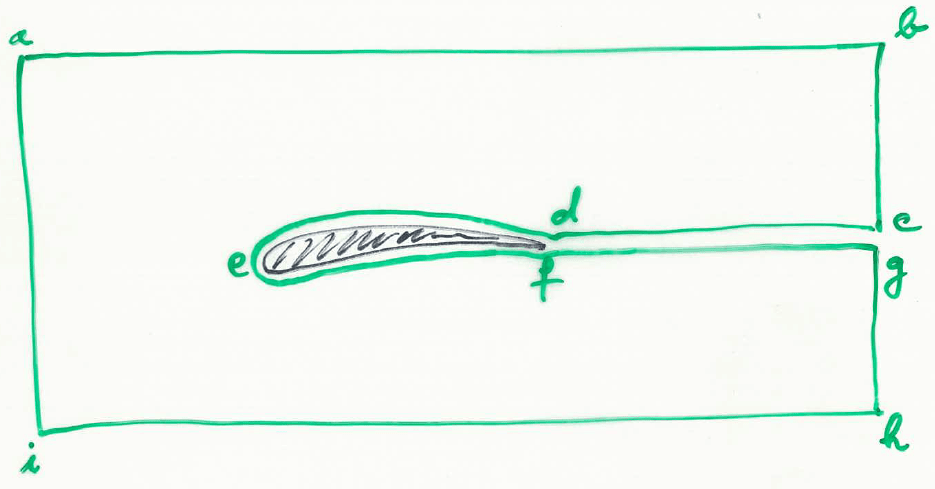
\includegraphics[scale=0.2]{ch1/1}
	\captionof{figure}{}
\end{wrapfigure}
When looking at an airfoil, we have a pressure that is applied around it. This pressure is non uniform, due to the presence of the airfoil. The integral of pressures over the surface gives a force expressed as the product of the incoming speed and the vorticity vector: the lift.

\subsection{Explain the origin of the bound vortex which exists around a profile which
	generates lift. Explain using the Kelvin theorem}
In inviscid case, the Kelvin theorem states that there cannot be vorticity, so no lift. If we take an arbitrary contour around the airfoil we will have no circultion. In inviscid case we can never get a lift $\rightarrow$ D’alembert paradox. At the trailing edge, if the flow wants to continue on the other corner from below, the velocity must be infinity so that the flow separates. But this is not the case in reality. \\

\begin{wrapfigure}[7]{r}{6.5cm}
	\vspace{-5mm}
	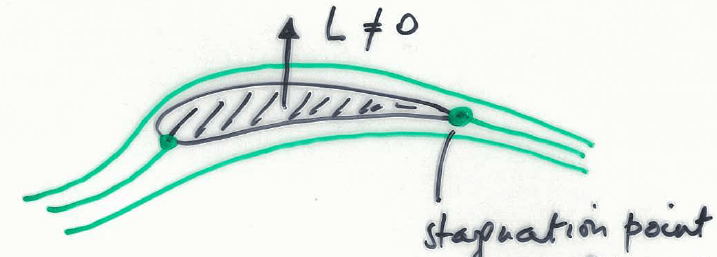
\includegraphics[scale=0.25]{ch1/4}
	\captionof{figure}{}\label{fig1}
\end{wrapfigure}
To satisfy the Kutta condition (the flow has to leave the airfoil smoothly), there needs to be circulation if we take a contour that contains the airfoil, but for all contour that does not contain the airfoil it is null.  $\Gamma$ varies with the stagnation point position, but only one corresponds to the Kutta condition. \\

\begin{wrapfigure}[16]{l}{4cm}
	\vspace{-5mm}
	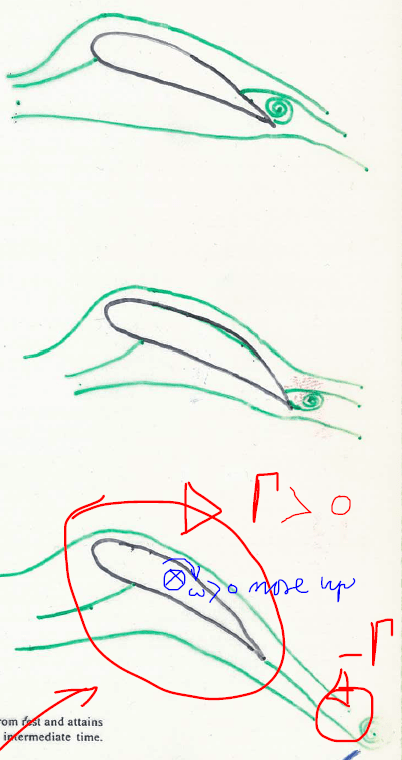
\includegraphics[scale=0.25]{ch1/5}
	\captionof{figure}{}
\end{wrapfigure}
The bound vortex is the vortex around the airfoil. It is compensated by a starting vortex that detaches from the airfoil.

We can show that every contour containing the airfoil has a non 0 circulation. Let's proof that a contour that doesn't contain the airfowl has $\Gamma =0$: 

\begin{equation}
\oint _{C} \vec{v}\, d\vec{l} = \oint _{\mbox{airfoil}} \vec{v}\, d\vec{l} + \oint _{cd} \vec{v}\, d\vec{l} + \oint _{fg} \vec{v}\, d\vec{l} = 0. 
\end{equation}

As the contour elements are exactly opposed to each other, the result is null. 

\subsection{What is the start-up vortex, what happens with it when the flow reaches a
	steady state}
What happens is that initially we have the first kind of flow, then the formation of the starting vortex due to viscous effects (separation) which is compensated by a \textbf{bound vortex} around the airfoil (to respect Kelvin theorem of irrotational flow) that makes $\Gamma \neq 0$. Then the vortex goes away to infinity. Indeed if we take $R = \rho v_\infty \Gamma$, $\Gamma \neq 0$, so we have lift. 
\subsection{Explain the Kutta condition}
The Kutta condition states that the flow can only have a stagnation point at the trailing edge. If this was not the case, the underwing flow would need to accelerate "going backwards" to meet the upperwing flow, see figure~\ref{fig1}.

%-----------------------------------------------------------------------------------------------------------------
%-----------------------------------------------------------------------------------------------------------------
%-----------------------------------------------------------------------------------------------------------------

\section{Derive an expression for the aerodynamic lift of on airfoil for inviscid
	incompressible flow (i.e. neglecting viscous effects).}

\begin{wrapfigure}[9]{l}{7.5cm}
	\vspace{-5mm}
	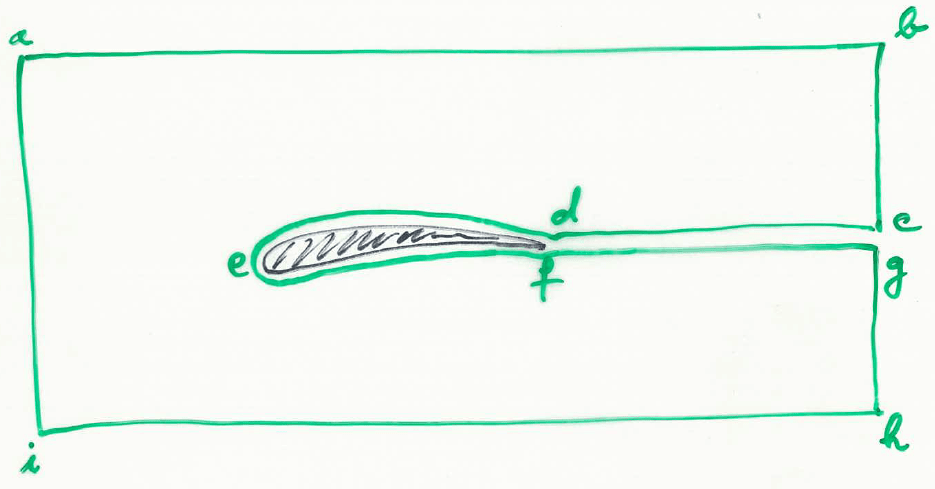
\includegraphics[scale=0.2]{ch1/1}
	\captionof{figure}{}
\end{wrapfigure}

The fundamental integral form of the mass conservation equation is:\\

\begin{equation}
\frac{d}{dt}\int _V \rho \, dV + \oint _S \rho \vec{v} \, d\vec{S} = 0.
\end{equation}

By applying Gauss theorem $\oint _S \vec{a}.\vec{n}\, dS = \int _V \nabla\vec{a}\, dV$:

\begin{equation}
\int _V \left[\frac{d \rho}{d t} + \nabla .(\rho \vec{v})\right]\, dV = 0. 
\end{equation}

True for all volumes:

\begin{center}
	\theor{
		\textbf{Continuity equation}
		\begin{equation}
		\frac{d \rho}{d t} + \nabla .(\rho \vec{u}) = 0
		\label{eq:1.3}
		\end{equation}
	}		
\end{center}

General form of the momentum equation is: 

\begin{equation}
\rho \dot{\vec{v}} = \frac{\D \rho \vec{v}}{\D t} + \rho (\vec{v}\nabla ) \vec{v} = -\nabla p + \nabla \bar{\bar{\tau}}.
\end{equation}

Steady state, time derivative goes away. If we consider the x component of the velocity, we can expend the derivative to the whole left term as:

\begin{equation}
\rho (\vec{v}\nabla ) v_x = \nabla (\rho \vec{v} v_x) - v_x \cancel{\nabla (\rho \vec{v})}
\label{eq:1.5}
\end{equation}

where the last term is null related to \eqref{eq:1.3} in steady state. Integrating both sides around the volume contained in the closed surface S (abcdefghi on figure) in \eqref{eq:1.5}, and applying Gauss theorem, we obtain:

\begin{equation}
\oint _{S} \vec{v} (\rho \vec{v} \vec{n}) \, dS = -\oint _{S} p \, d\vec{S} + \oint _{S} \bar{\bar{\tau}} \, d\vec{S}.
\label{eq:1.6}
\end{equation}		 

New closed contour $S* = S - \mbox{airfoil} - cd - fg$ (previous abhi in fact). \eqref{eq:1.6} becomes:

\begin{equation}
\begin{aligned}
&\oint _{S^*} \vec{v} (\rho \vec{v} \, d\vec{S})  + \cancel{\oint _{\mbox{airfoil}} \vec{v} (\rho \vec{v} \, d\vec{S})} + \cancel{\oint _{cd+fg} \vec{v} (\rho \vec{v} \, d\vec{S})} 
\\&= -\oint _{S^*} p \, d\vec{S} -\oint _{\mbox{airfoil}} p \, d\vec{S}-\cancel{\oint _{cd + fg} p \, d\vec{S}}+ \oint _{S^*} \bar{\bar{\tau}} \, d\vec{S} +\oint _{\mbox{airfoil}} \bar{\bar{\tau}}\, d\vec{S} +\cancel{\oint _{cd + fg} \bar{\bar{\tau}}\, d\vec{S}}
\end{aligned}
\label{eq:1.7}
\end{equation}

Forces applied to a wing:
\begin{equation}
\vec{R} = \oint _{\mbox{airfoil}} p\, d\vec{S} - \oint _{\mbox{airfoil}} \bar{\bar{\tau}}\, d\vec{S}	
\end{equation}

\begin{equation}
\oint _{S^*} \vec{v} (\rho \vec{v} \, d\vec{S}) = -\oint _{S^*} p \, d\vec{S} + \cancel{\oint _{S^*} \bar{\bar{\tau}} \, d\vec{S}} - \vec{R}.
\label{eq:1.9}
\end{equation}

Pressure effects induced by the body remains at a long distance from the body. We have to analyse the \textbf{non uniform} p along S*. In order to apply Bernouilli equation $p + \frac{1}{2}\rho v^2 = cst$, let's add the constants $p_\infty$ and $v_\infty$ to \eqref{eq:1.9}, as $\oint p_\infty\, d\vec{S} = p_\infty \oint d\vec{s} = 0$: 

\begin{equation}
\vec{R} = -\oint _{S^*} (p-p_\infty) \, d\vec{S} - \oint _{S^*} (\vec{v}-\vec{v}_\infty) \, d\dot{m}
\label{eq:1.12}
\end{equation}

Let's express $\vec{v} = \vec{v}_\infty + \vec{\delta _c}$ with $\vec{\delta _c}$ a perturbation. Introducing this in Bernouilli equation: 

\begin{equation}
\begin{aligned}
p_\infty +\frac{1}{2} \rho \cancel{\vec{v}_\infty ^2} = p + \frac{1}{2} \rho( &\vec{v}_\infty + \vec{\delta _c})^2 = p + \frac{1}{2} \rho (\cancel{\vec{v}_\infty ^2} + 2 \vec{v}_\infty \vec{\delta _c} + \cancel{\vec{\delta _c}^2}) \\
&\Rightarrow p-p_\infty = - \rho\vec{v}_\infty \vec{\delta _c}	.		
\end{aligned}
\end{equation}

If we replace this result in \eqref{eq:1.12}, we find:

\begin{equation}
\vec{R} =\oint _{S^*} \rho [(\vec{v}_\infty \vec{\delta _c}) \, d\vec{S} - \vec{\delta _c} [(\vec{v}_\infty . d\vec{S})]
\end{equation}

by using a vector property $\vec{a} \times (\vec{b} \times \vec{c}) = (\vec{a} \vec{b})\vec{c} - (\vec{a}\vec{c})\vec{b}$:

\begin{equation}
= \rho \vec{v}_\infty \times \oint _{S^*} \vec{\delta _c} \times d\vec{S} = \rho \vec{v}_\infty \times \left[\oint _{S^*} \vec{v} \times d\vec{S} - \cancel{\oint _{S^*} \vec{v}_\infty \times d\vec{S}}\right]
\end{equation}

and by applying Stokes theorem $\oint _S \vec{a} \times d\vec{S} = \int _V \nabla \times \vec{a} \, dV$:

\begin{equation}
= \rho \vec{v}_\infty \times \int  (\nabla \times \vec{v})\, dV = \rho \vec{v}_\infty \times \int  \vec{\omega}\, dV
\end{equation}

where $\vec{w}$ is the \textbf{vorticity vector} of direction $\vec{1}_z$ (pointing in the paper):

\begin{equation}
\vec{\omega} = 
\left| \begin{array}{ccc}
\vec{1}_x & \vec{1}_y & \vec{1}_z \\ 
\D _x & \D _y & 0 \\ 
v_x & v_y & 0
\end{array} 
\right| 
= [\D _x v_y - \D _y v_x] \vec{1}_z
\end{equation}

This shows that the lift force is always perpendicular to the flow!


\subsection{Express conservation of momentum over a closed surface S far away from
	the wing, neglecting viscous forces}
\begin{wrapfigure}[11]{l}{6.5cm}
	\vspace{-5mm}
	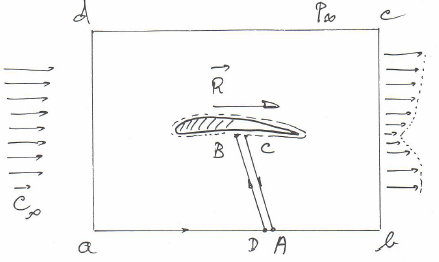
\includegraphics[scale=0.4]{ch1/2}
	\captionof{figure}{}
\end{wrapfigure}
By considering this (assumption of far field), we can compute the force only by knowing the far field parameters. Indeed, uniform pressure implies null surface integral, so that \eqref{eq:1.9} becomes:

\begin{equation}
\vec{R} = -\oint _{S^*} \vec{v} (\rho \vec{v} \, d\vec{S}).
\end{equation}

The velocity term remains, as by experience we know that there is a \textbf{wake} making the velocity profile non-uniform. Let's now consider that the velocity is horizontal so that $\vec{R} = R.\vec{1}_x$, at the inlet we have $\vec{v}$ and $\vec{n}$ are opposed while at the outlet they are in the same direction: 

\begin{equation}
\vec{R} = \int _a^d \vec{v}\, d\dot{m} - \int _b^e \vec{v}\, d\dot{m} > 0
\end{equation}

showing that there is only \textbf{drag} force.

\subsection{Show that the lift force is linked to the vorticity through the closed surface S}
See above.
\subsection{Show that for the 2D airfoil the lift force is linked to the circulation around
	the airfoil, derive the Kutta-Joukowski formula for the lift generated by a 2D
	profile}

We will now introduce the circulation $\Gamma = - \oint \vec{v} \, d\vec{l} >0$   around a body. The convention is to take the anticlockwise direction for $d\vec{l}$ and so for $\Gamma$ to be $>0$ we must have $\vec{v}$ in the clockwise direction. There is a link between the lift force and the circulation. Let's introduce \textbf{Stokes theorem}:

\begin{equation}
\oint \vec{a} d\vec{l} = \int _S (\nabla \times \vec{a})\, d\vec{S} \qquad \Rightarrow -\Gamma = \int _S \vec{\omega} d\vec{S}.
\end{equation}

We remember that:
\begin{equation}
\begin{aligned}
\vec{R} &= \rho \vec{v}_\infty \times \int  \vec{\omega}\, dV = \rho \vec{v}_\infty \times \int  l\vec{\omega}\, dS \qquad \Leftrightarrow \frac{\vec{R}}{l} = \rho \vec{v}_\infty \times \int  \vec{\omega}\, dS \\
\frac{\vec{R}}{l}&= \rho \vec{v}_\infty \times \int  \vec{\omega}\, (d\vec{S}.\vec{1}_z) = \rho \vec{v}_\infty \times (-\Gamma)\vec{1}_z = \rho v_\infty \Gamma \,\vec{1}_y
\end{aligned}
\end{equation}

to finally obtain a very good approximation of the lift:

\begin{center}
	\theor{
		\textbf{Kutta formula for lift 2D airfoil}
		\begin{equation}
		|R| = \rho v_\infty \Gamma 
		\end{equation}
	}
\end{center}


%-----------------------------------------------------------------------------------------------------------------
%-----------------------------------------------------------------------------------------------------------------
%-----------------------------------------------------------------------------------------------------------------

\section{Characteristics of a 2D airfoil:}
\subsection{Define lift and drag, give the principle components of lift and drag force in
	normal operation and in case of separation}
	
\begin{wrapfigure}[9]{l}{7.5cm}
	\vspace{-5mm}
	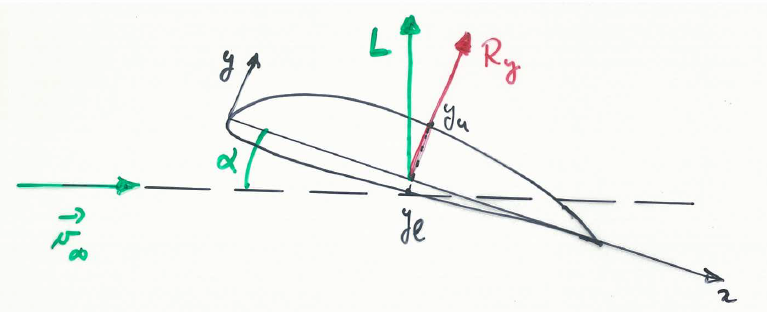
\includegraphics[scale=0.25]{ch2/3}
	\captionof{figure}{}
	\label{fig:2.2}
\end{wrapfigure}
Force applied on the wing:

\begin{equation}
\vec{R} = -\oint p \, d\vec{S} + \oint \bar{\bar{\tau}} \, d\vec{S} 
\end{equation}

with an external normal to the airfoil. The angle of attack is represented on \autoref{fig:2.2}.

The pressure term is responsible for lift and the friction term is responsible for drag. Friction forces work tangential to the airfoil and the pressure forces are perpendicular, if there is \textbf{no separation} in the flow. The drag created by the stress is called the \textbf{skin} or \textbf{friction} drag. 
Note that in a subsonic inviscid incompressible flow, we have the paradox of d’Alembert because we have no drag. This shows that the pressure only contributes to lift. \\

\textbf{Separation}: region above the airfoil where $p-p_\infty \approx 0$ $\Rightarrow$high pressure below $p\gg p_\infty$ that slows down the wing. This implies that the applied force is higher than the case without separation and due to the attack angle, the drag force too. This phenomenon is called \textbf{pressure drag} (form drag), and here the pressure contributes to drag.


\subsection{Explain the non-dimensional force coefficients($C_l$, $C_d$, $C_m$) and which are the
	similarity parameters influencing these coefficients}
Let’s look to the non-dimensional parameters that will influence the lift, the drag and the momentum. We have to define some reference quantities: 

\begin{equation}
\begin{array}{cccc}
L_{ref} = C & v_{ref} = v_\infty & t_{ref} = L_{ref}/v_{ref} & \rho _{ref} = \rho _\infty \\
t’= t/t_{ref} & p_{ref} = \rho _{ref} \frac{v_{ref} ^2}{2} & \mbox{Mach} = V_{ref} / a_{ref} & a_{ref} = \gamma \pi T_{ref} \\
\gamma = c_p / c_v && Re_{ref} = \frac{\rho _{ref} v_{ref} L_{ref}}{\mu _{ref}} &
\end{array}
\end{equation}					

where $a$ is the speed of sound. By replacing all these in the mass, momentum and energy equations, we obtain the non-dimensional ones (see Fluid Mechanics II):

\begin{equation}
\begin{aligned}
&\bullet\frac{\D \rho '}{\D t'} + \nabla \left(\rho ' \vec{v}'\right) = 0\\
&\bullet\rho ' \frac{d\vec{v}'}{dt'} = - \frac{1}{\gamma M^2_{ref}}\nabla p' + \frac{1}{\mbox{Re}_{ref}}\nabla \bar{\bar{\tau}'}\\
&\bullet\frac{d}{dt'}(\rho ' e')+ \frac{\gamma (\gamma -1)}{2} M^2_{ref}\frac{d}{dt'}(\rho ' \vec{v'}^2 ) \\
&= \frac{\gamma}{Pr_{ref}Re_{ref}} \nabla (k'\nabla T') - (\gamma -1)\nabla (p'\vec{v}')+ \gamma (\gamma -1) \frac{M_{ref}^2}{Re_{ref}} \nabla (\bar{\bar{\tau}}'\vec{v}')			\end{aligned}
\end{equation}

We can see that a solution can only be function of 4 parameters: $M, Re, Pr = \frac{c_p \mu}{k}, \gamma$, but we know that the geometry and the angle of attack $\alpha$ have a role by means of the boundary conditions. Then, we assume that the fluid is air ($\gamma =1.4$) and that we can neglect heat effects (no influence of Pr, incompressible and so low speed flows). The non-dimensional lift, drag and moment are thus function of M, Re, geometry and $\alpha$. We can define \textbf{lift}, \textbf{drag} and \textbf{moment coefficient} as (we forget about compressibility $\rightarrow$ M, and Re effects are low for $C_L and C_M$): 

\begin{equation}
\begin{aligned}
&C_L(\cancel{M}, \cancel{Re}, geometry, \alpha) = \frac{L}{\frac{1}{2}\rho _{ref} v^2_{ref} S} \\
&C_D(\cancel{M},Re, geometry, \alpha) = \frac{D}{\frac{1}{2}\rho _{ref} v^2_{ref} S}		\\
&C_M(\cancel{M}, \cancel{Re}, geometry, \alpha) = \frac{M}{\frac{1}{2}\rho _{ref} v^2_{ref} Sc}
\end{aligned}	
\label{eq:2.18}		
\end{equation}

where L, D, M are the \textbf{dimensional} forces, c the mean chord (S/b) and S a reference surface (3D wing $\rightarrow$ total wing surface, 2D wing $\rightarrow$ S = c). We can experimentally show that the lift increases mainly linearly with $\alpha$ and the drag force is caused by friction effects and pressure differences involving with $\alpha$. This gives the following equations (lower case for 2D):

\begin{equation}
c_l = m(\alpha - \alpha _{L_0}) \qquad c_d = c_{d_0} + kc^2_l
\end{equation}

where $m\approx 2\pi$ theoretically and 5.7 practically, k is a constant of order of magnitude 0.01.

\subsection{Explain:}
\textbf{center of pressure CP:} It's the x value on the chord where the carrier of the force $\vec{R}$ intersects the chord. It's function of the angle of attack. Indeed, if alpha increases, the suction peak will be higher, this induces that the center of pressure move forward (participation of the forward pressure more important).\\

Note that the center of pressure is not a fixed point. Indeed, it varies with the angle of attack: if $\alpha \nearrow$, the pressure peak on the LE is more important making the $x_p$ move upstream, and the contrary for $\alpha \searrow$. This notion will be completed by the \textbf{zero lift angle} $\alpha _{0}$.

\textbf{equivalent force system in an arbitrary point Q on the chord of the profile:} 
\begin{wrapfigure}[7]{l}{3cm}
	\vspace{-5mm}
	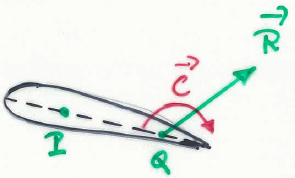
\includegraphics[scale=0.3]{ch2/11}
	\captionof{figure}{}
\end{wrapfigure}
The force at the pressure center P is equivalent to another force in point Q, but by adding the moment to compensate the one added by moving the force. This moment is:

\begin{equation}
\vec{C_Q} = -\vec{PQ}\times \vec{R}.
\end{equation}
\textbf{aerodynamic center AC:} Suppose that there is a point Q where the couple $C_Q$ is independent of the angle of attack (because the pressure center changes with alpha). This point is called the aerodynamic center.

The moment at this point is always nose-down and the point is situated upstream to the center of pressure.

\textbf{the graph of the momentum coefficient $c_m$ at a point Q versus the
	lift coefficient $c_l$ for Q located at the trailing edge, at the leading edge and at
	the aerodynamic center of the profile:} It is shown experimentally that:

\begin{equation}
c_m(Q) = c_{m_0} + k c_l
\label{eq:2.11}
\end{equation}

\begin{center}
	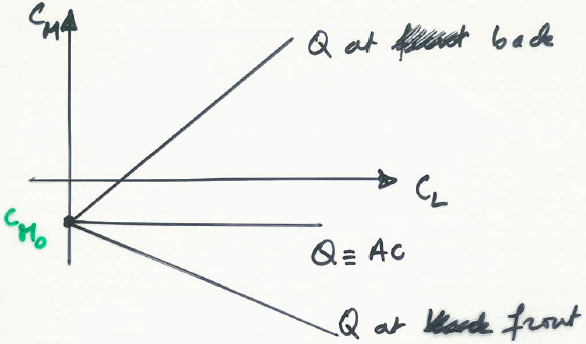
\includegraphics[scale=0.23]{ch2/14}
	\captionof{figure}{}
\end{center}
$k$ is a constant that is related to the reference point chosen. If $Q$ is taken on the LE for example, increasing $\alpha$ will produce an increase of the lift and make the center of pressure move upstream. The L increase will compensate the moving $x_p$ such that the moment becomes even more noose-down (more negative following $\vec{1}_z$) $\Rightarrow k<0$ for a decrease in \eqref{eq:2.11}. The same reasoning applied on the trailing edge gives $k>0$. 
\subsection{Compute the Location of the center of pressure CP as a function of the angle of
	attack alpha}
\begin{equation}
\begin{array}{cccc}
1) & c_m = c_{m_0} + kc_l & 2)& M_{ac} = (x_{ac}-x_{cp})N \\
3) & m_{ac} = M_{AC} = M_0 <0 & 4) & N = n(\alpha-\alpha _0)
\end{array}
\end{equation}

The AC being always upstream the CP the difference in 2) is $<0$. In 4), $n>0$. By using equation 3,4 and 2, we can compute:

\begin{equation}
M_0 = -(x_{cp}-x_{ac}).n(\alpha - \alpha _0) \quad \Leftrightarrow \quad -\frac{M_0}{n} = (x_{cp}-x_{ac}).(\alpha - \alpha _0)
\end{equation}


\begin{wrapfigure}[8]{l}{4.5cm}
	\vspace{-5mm}
	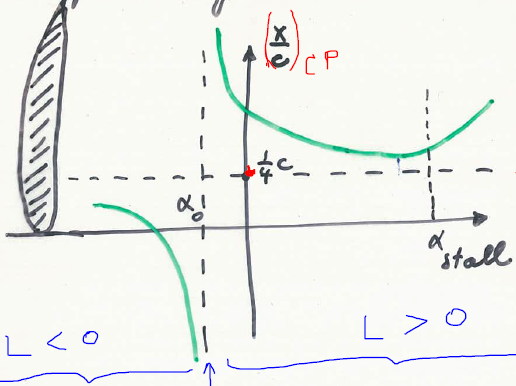
\includegraphics[scale=0.2]{ch2/17}
	\captionof{figure}{}
\end{wrapfigure}
This is the equation of an \textbf{hyperbola}. To see it, we only have to compute the limits of:

\begin{equation}
\begin{array}{c}
x_{cp} = x_{ac} - \frac{M_0}{n}\frac{1}{\alpha - \alpha _0}\\
\lim _{\alpha \rightarrow \pm\infty} x_{cp} = x_{ac} \qquad \lim _{\alpha \rightarrow \alpha _0 >0} x_{cp} = +\infty \qquad \lim _{\alpha \rightarrow \alpha _0 <0} x_{cp} = -\infty
\end{array}
\end{equation}

Let's finally say that commonly, $x_{ac} = cst \approx \frac{1}{4}C$.
\subsection{Explain the lift, drag and moment curves as a function of the angle of attack alpha}
Starting from what is said in 3.2, experiment showed that lift is increasing linearily with $\alpha$, and drag goes proportionnaly to $c_l^2$. The moment is proportionnal to $c_l$, we thus expect it to be linear with respect to $\alpha$.

\subsection{Explain what is stall and critical angle of attack. Explain different types of stall.}
\begin{wrapfigure}[11]{l}{6cm}
	\vspace{-5mm}
	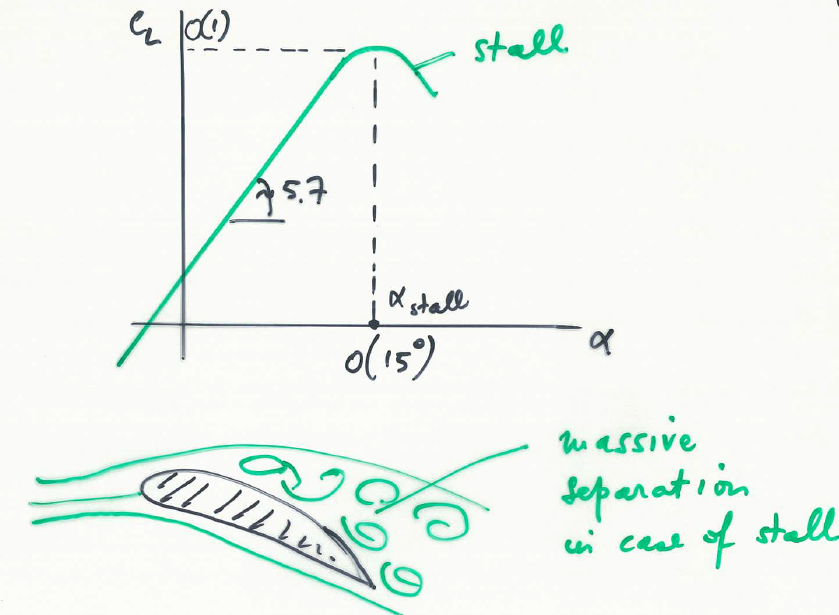
\includegraphics[scale=0.16]{ch2/18}
	\captionof{figure}{}
\end{wrapfigure}
At a certain angle of attack ($\approx 15\degres$), the lift suddenly drops. This is due to massive separation on the suction side (reverse pressure gradient too high) and happens at the \textbf{critical angle of attack}. This phenomenon is called \textbf{stall}. In the separated part, the pressure will no longer decrease and will form a pressure plateau. \\

We have to make the difference between leading-edge stall and trailing-edge stall. For \textbf{leading-edge stall}, the massive separation occurs suddenly near the LE resulting \newpage

\begin{wrapfigure}[13]{r}{5.7cm}
	\vspace{-5mm}
	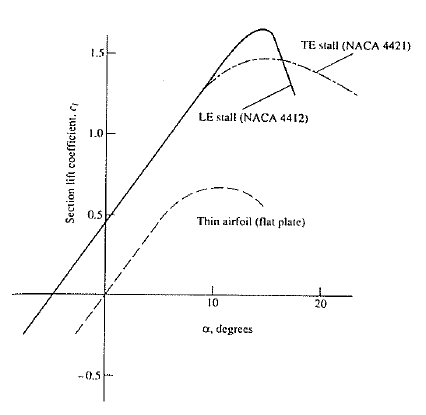
\includegraphics[scale=0.4]{ch2/19}
	\captionof{figure}{}
\end{wrapfigure}
in a strong and sudden drop of lift, when at maximum lift. This especially occurs to thin airfoils with cross-sections between 10 and 16\% of the chord. For the \textbf{trailing-edge stall}, the point of separation gradually goes upstream with increasing angle of attack resulting in a more gradual drop of lift (more thick airfoils). The comparison is done on the right figure. We can also see a third type of stall called \textbf{thin airfoil stall} with the example of a flat plat.  \\

In conclusion, the LE must be sufficiently rounded to have a good maximum lift. In fact the profile may nor be too 

\begin{wrapfigure}[8]{l}{7cm}
	\vspace{-5mm}
	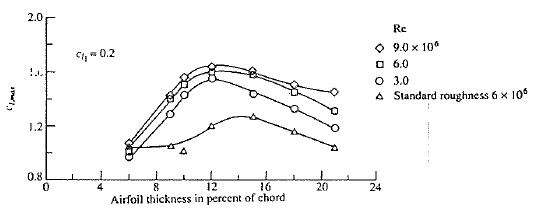
\includegraphics[scale=0.4]{ch2/20}
	\captionof{figure}{}
\end{wrapfigure}
thick  nor too thin. The figure on the left shows the influence of the thickness on the lift. We notice that the optimum thickness is situated around 12\% of the chord.The maximum lift increases with RE, indeed higher the Re, higher is the ratio of speed versus viscosity. So we can better oppose to separation. Unlike the Re number, the roughness has great effects on the maximum lift. Finally, let's notice that the camber have also an effect on maximum lift, the best is a camber of 8 up to 10\%.

\begin{equation}
L = C_L \frac{1}{2} \rho _{ref} v^2_{ref} S.
\label{eq:2.21}
\end{equation}

The lift force must always at least be equal to the weight of the plane. This implies that for low speed (take-off and landing), the $C_L$ must be large. This is accomplished with large $\alpha$ and slats or flaps. The minimum speed where the lift can still balance the weight ($C_L$ maximum) is called \textbf{stall speed} and from \eqref{eq:2.21} we find:

\begin{equation}
v_{stall} = \sqrt{\frac{W}{C_{L_{max}} \frac{1}{2} \rho_{ref} S}}
\end{equation}

\subsection{Discuss the polar curve of the airfoil, i.e. lift coefficient as a function of drag
	coefficient, show the glide ratio on this plot}
\begin{wrapfigure}[10]{r}{4cm}
	\vspace{-5mm}
	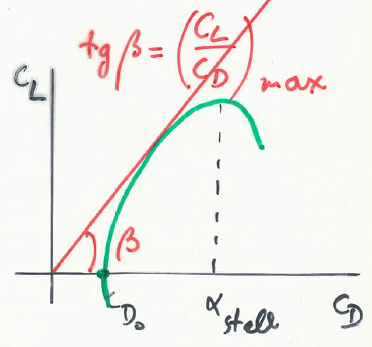
\includegraphics[scale=0.3]{ch2/21}
	\captionof{figure}{}
\end{wrapfigure}
The curve that represents $C_L$ in function of $C_D$ is the \textbf{polar curve} of the wing. The ratio $\frac{C_L}{C_D}$ is the \textbf{glide ratio} or \textbf{finesse} and is like an efficiency parameter. 
\subsection{What is the importance of the glide ratio, discuss the case of a gliding plane
	(engine off situation)}
The best parameter is obtained using the graph by calculating $\beta$ such that: 

\begin{equation}
\tan \beta = \left(\frac{C_L}{C_D}\right)_{max}
\end{equation}						

This point is important for the quality of the wing because if we plot the thrust, the lift, the drag and the weight of a plane describing a horizontal flight (\autoref{fig:2.21}), the thrust is given by:

\begin{equation}
T = \frac{L}{\tan \beta} = \frac{W}{\tan \beta}
\end{equation}

where we see that when $\tan \beta$ (so the glide ratio) increases, T decreases. Another interpretation can be given when we have no thrust (\autoref{fig:2.22}). In this case the gliding ratio has to be adapted to travel the larger distance knowing that:

\begin{equation}
\frac{C_L}{C_D} = \frac{\mbox{distance travelled}}{\mbox{height loss}}
\end{equation}

\begin{center}
	\begin{minipage}{0.3\textwidth}
		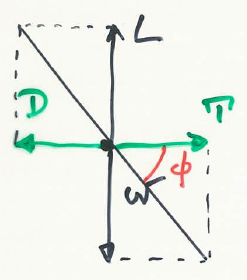
\includegraphics[scale=0.5]{ch2/22}
		\captionof{figure}{}			
		\label{fig:2.21}
	\end{minipage}
	\begin{minipage}{0.5\textwidth}
		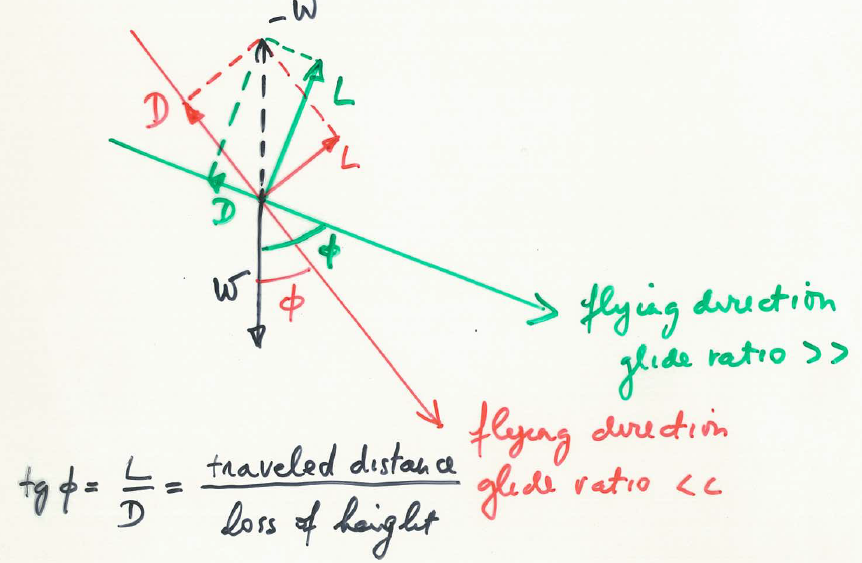
\includegraphics[scale=0.2]{ch2/23}
		\captionof{figure}{}			
		\label{fig:2.22}
	\end{minipage}
\end{center}
%-----------------------------------------------------------------------------------------------------------------
%-----------------------------------------------------------------------------------------------------------------
%-----------------------------------------------------------------------------------------------------------------

\section{Computation of inviscid irrotational flow around a 2D airfoil using conformal
	mapping - Joukowski profiles}
\subsection{Explain methods based on complex potential function, explain the
	connection with usual stream function and potential function}
We will begin here with steady, inviscid irrotational flows. This gives for the mass conservation equation:

\begin{equation}
\frac{\D \rho}{\D t} + \nabla (\rho \vec{v}) = 0 \qquad \Rightarrow \nabla \vec{v} = 0 = \D _x u + \D _y v
\end{equation}

In the other hand, we have the assumption of irrotational flow:

\begin{equation}
\vec{\omega} = 0 \qquad \Rightarrow \D _x v - \D _y u = 0.
\end{equation}

Then we define the \textbf{complex potential function w}:

\begin{equation}
w = \phi + I\psi
\end{equation}		 

where $\phi$ is the \textbf{potential function} (satisfies $w=0$ by construction) such that:

\begin{equation}
\left\{
\begin{aligned}
&u = \D _x \phi \\
&v = \D _y \phi
\end{aligned}
\right.
\qquad
\nabla \phi = \vec{v} = \D _x\phi \vec{1} _x + \D _y \phi \vec{1}_y
\end{equation}

We must satisfy the mass conservation equation:
\begin{equation}
\nabla (\nabla \phi) = 0 \qquad \Rightarrow \Delta \phi = 0 
\end{equation}

coupled with boundary conditions, we can find a solution $\phi (x,y)$. The \textbf{stream function} satisfies the mass conservation by construction:

\begin{equation}
\left\{ 
\begin{aligned}
&u = \D _y \psi\\
&v = - \D _x \psi
\end{aligned}
\right.
\qquad \Rightarrow \D _x u + \D _y v = 0 \Leftrightarrow \D _x (\D _y \psi) + \D _y (- \D _x \psi) = 0
\end{equation}

\begin{wrapfigure}[8]{l}{4cm}
	\vspace{-5mm}
	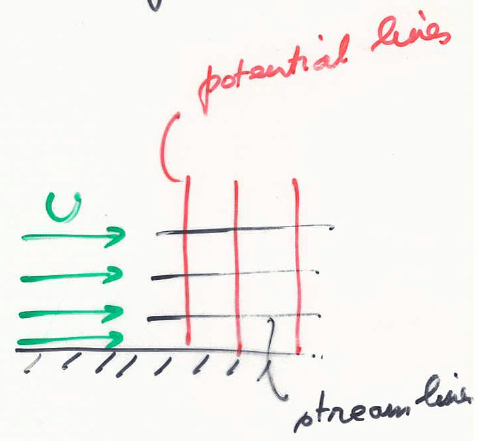
\includegraphics[scale=0.2]{ch2/24}
	\label{fig:2.23}
	\captionof{figure}{}
\end{wrapfigure}
We still have to verify the $\omega=0$ condition:
\begin{equation}
\D _x v - \D _y u = 0 \qquad \Rightarrow \frac{\D ^2 \psi}{\D x^2} + \frac{\D ^2 \psi}{\D y^2} = 0 \qquad \Delta \psi = 0
\end{equation}
A streamline and a potential line are perpendicular to each other:
\begin{equation}
\nabla \psi . \nabla \phi = \D _x \psi \D _x \phi + \D_ y \psi \D _y \phi = -vu + uv = 0. 
\end{equation}

	Analytical means differentiable. This consist in defining a function $f(z)$ analytical such that:

\begin{equation}
w = f(z) \qquad z,\omega \in \mathbb{C} \qquad \Rightarrow w = \phi +i \psi \qquad \left\{
\begin{aligned}
&z= x+iy\\ 		 
&\phi = \phi (x,y) \in \mathbb{R}\\
&\psi =  \psi(x,y) \in \mathbb{R}
\end{aligned} 		  
\right.
\end{equation}

If this is differentiable everywhere, $\Delta \phi = \Delta \psi = 0$. 

\subsection{Explain how the velocity can be computed from the complex potential
	function}

The complex velocity (velocity field):

\begin{equation}
\frac{dw}{dz} = \frac{df}{dz} = A + iB \qquad A = \frac{\D \phi}{\D x} = - \frac{\D \psi}{\D y} = u \quad B = \frac{\D \psi}{\D x} = - \frac{\D phi}{\D y} = -v
\end{equation}

A property of this $f(z)$ is the superposition principle: $w_1 = f_1(z), w_2 = f_2(z)$ so $w_1 + w_2 = f_1(z)+f_2(z)$.
\subsection{Derive the complex potential function for uniform flow, source/sink flow,
	free vortex}
\subsubsection{Uniform flow}

\begin{equation}
w = U z \qquad \frac{d w}{dz} = U = u+iv \qquad \Rightarrow u = U; v = 0
\end{equation}

\subsubsection{Source / Sink}
\begin{wrapfigure}[8]{r}{3cm}
	\vspace{-5mm}
	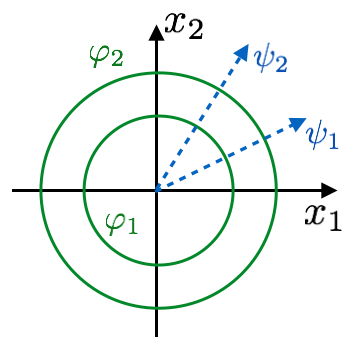
\includegraphics[scale=0.3]{ch2/25}
	\captionof{figure}{}
\end{wrapfigure}
In this case, using the cylindrical coordinates, the complex potential is defined as ($\Lambda$ being the volumetric flow): 

\begin{equation}
\begin{aligned}
&w = \frac{\Lambda}{2\pi} \ln z = \frac{\Lambda}{2\pi} \ln (r e^{i\theta}) = \frac{\Lambda}{2\pi} (\ln r + i\theta) \\
&\Rightarrow \phi = \frac{\Lambda}{2\pi} \ln r, \psi =  \frac{\Lambda}{2\pi}\theta.
\end{aligned}
\end{equation}

We see that complex lines corresponds to $r =cst$ so are circles and streamlines $\theta = cst$ are line of constant angle. $\oint \vec{v}\, d\vec{l}=0$ as velocity is everywhere tangent to any circular contour. Let's compute the derivative for the velocity field:

\begin{equation}
\frac{dw}{dz} = \frac{\Lambda}{2\pi z} = \frac{\Lambda (x-iy)}{2\pi (x^2+y^2)} = \frac{\Lambda}{2\pi r} (\cos \theta - i \sin \theta).
\end{equation}

We see that the velocity decreases in $1/r$, this is due to the constant mass flow, so if the surface increases with r the velocity has to decrease to keep $\dot{m} = \rho v S$ constant. 

\subsubsection{Free vortex}
\begin{wrapfigure}[5]{l}{3cm}
	\vspace{-5mm}
	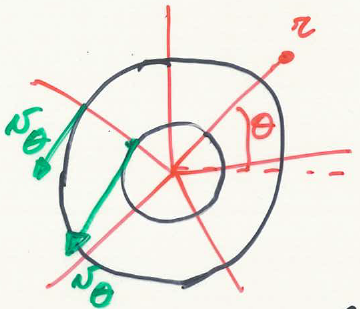
\includegraphics[scale=0.23]{ch2/26}
	\captionof{figure}{}
\end{wrapfigure}
We do the same as the other cases: 
\begin{equation}
\begin{aligned}
&w = \frac{i\Gamma}{2\pi} \ln z = \frac{i\Gamma}{2\pi} \ln (re^{i\theta}) = \frac{i\Gamma}{2\pi} (\ln r + i\theta) = -\frac{\Gamma}{2\pi} \theta + \frac{i\Gamma}{2\pi} \ln r \\
&\phi = -\frac{\Gamma}{2\pi} \theta, \psi = \frac{\Gamma}{2\pi} \ln r
\end{aligned}
\end{equation}

We see that this is the inverse case of the previous one, streamlines are circles oriented in negative rotational motion around z-axis (z entering in the sheet) so clockwise. We can compute the velocity field by deriving among z and we find that: 

\begin{equation}
u = \frac{\Gamma \sin \theta}{2 \pi r} \qquad v = -\frac{\Gamma \cos \theta}{2\pi r}
\end{equation}

Let's specify that $v_\theta = \frac{1}{r} \frac{\D \phi}{\D \theta} = -\frac{\Gamma}{2 \pi r}$, and that we have a vortex singularity in the center because $\Gamma = 0. \infty$.

\subsection{Compute flow around Rankine body and around a cylinder}

	\begin{wrapfigure}[5]{r}{5.5cm}
	\vspace{-5mm}
	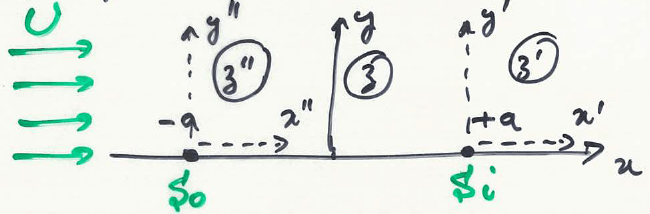
\includegraphics[scale=0.23]{ch2/27}
	\captionof{figure}{}
\end{wrapfigure}
Let's make a combination of a uniform flow and a source + sink as shown on the figure. The combination gives:

\begin{equation}
w = Uz + \frac{\Lambda}{2\pi} \ln \frac{z+a}{z-a}= Uz + \frac{\Lambda}{2\pi} \ln \frac{1+a/z}{1-a/z}.
\end{equation}

To have the flow around a cylinder we need to compute the limit $a\rightarrow 0$, and will need the Taylor expansion of $\ln$:

\begin{equation}
\ln \frac{1+\epsilon}{1-\epsilon} \approx 2 \epsilon + \cancel{o(\epsilon ^3)} \qquad \Rightarrow \lim _{a\rightarrow 0} w = \lim _{a \rightarrow 0} \left[ Uz + \frac{\Lambda}{2\pi} 2 \frac{a}{z} \right]
\end{equation}

by defining $\mu = 2\Lambda a$ we find the \textbf{flow around a cylinder}:

\begin{equation}
w = Uz + \frac{\mu }{2\pi z}.
\label{eq:2.42}
\end{equation}

If we replace $z= x+iy$ to find $\phi$ and $\psi$ we find:

\begin{equation}
\phi = Ux + \frac{\mu}{2\pi }\frac{x}{r^2} \qquad \psi = Uy - \frac{\mu }{2\pi} \frac{y}{r^2}.
\end{equation}

In this flow a closed streamline exists forming the so called \textbf{Rankine body} and which describes a cylinder in the case $a\rightarrow 0$. Indeed it is possible to find an exact solution for $\psi = 0$. This configuration has a symmetry according to x and y-axis when taking the center of the cylinder as origin. This implies that $\vec{F} = - \oint _{cyl} p\, d\vec{S} = 0$. This is the so called \textbf{paradox of d'Alembert} because we expect to find at least a drag force. A lift force can be find on the cylinder by adding a vortex. We conclude by saying that we can rewrite \eqref{eq:2.42} as (R the radius of the cylinder):

\begin{equation}
w = U\left( z + \frac{R^2}{z} \right) \qquad with \ R^2 = \frac{\mu }{2\pi U}.
\end{equation}

\subsection{Explain how a the class of Joukowski profiles is obtained by conformal
	mapping of a circle}
\begin{wrapfigure}[5]{l}{5.5cm}
	\vspace{-5mm}
	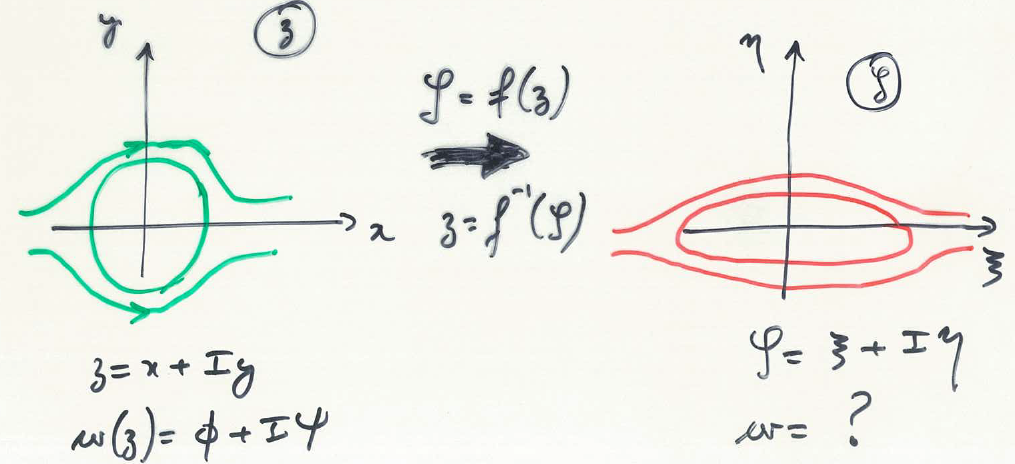
\includegraphics[scale=0.1]{ch2/28}
	\captionof{figure}{}
\end{wrapfigure}
Let's do a mapping, a transformation, to try to find our airfoil based on simple geometries. Let's as first example apply the transformation $Z = z + \frac{R^2}{z}$ to the cylinder of radius R. Let's first remark that the cylinder will become a flat plate:

\begin{equation}
Z = z + \frac{R^2}{z} = Re^{i\theta}  \frac{R^2}{Re^{i\theta}} = 2 R \cos \theta 
\end{equation}

Indeed, as $\cos \theta \in [-1,1]$ and the result is real, we have a flat plate between -2R and 2R in the x-axis. The flow Z is directly found: $W(Z) = UZ$. The second example will be the application of the same transformation on a cylinder of this time radius $r>R$. In this case the circle becomes an ellipse:

\begin{equation}
Z = r e^{i\theta} + \frac{R^2}{r^2}e^{-i\theta} = \left( r + \frac{R^2}{r} \right)\cos \theta + i \left( r - \frac{R^2}{r} \right) \sin \theta.
\end{equation}		 

Let's also compute the velocity field using the chain rule:

\begin{equation}
\frac{dW}{dZ} = \frac{dw}{dZ} = \frac{dw}{dz}\frac{dz}{dZ} = \left( 1 -\frac{r^2}{z^2} \right) \left( \frac{1}{1-\frac{R^2}{z^2}} \right).
\end{equation}

We see that the expression becomes infinite when $z^2 = R^2$. The reason is that the transformation is not analytical in these points so they must not be in the flow. 

The examples are summarized in the figures below 

\begin{center}
	\begin{minipage}{0.45\textwidth}
		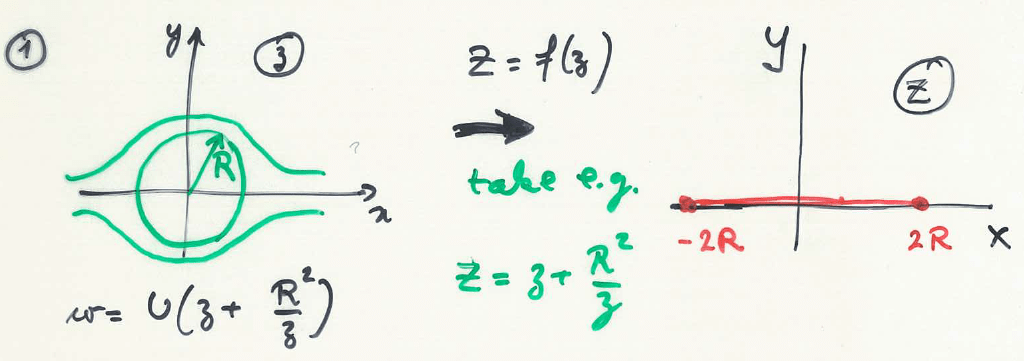
\includegraphics[scale=0.15]{ch2/29}
		\captionof{figure}{}
	\end{minipage}
	\begin{minipage}{0.45\textwidth}
		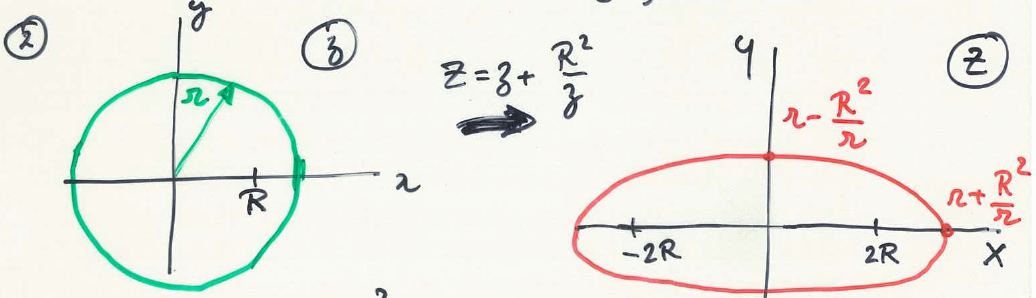
\includegraphics[scale=0.2]{ch2/30}
		\captionof{figure}{}
	\end{minipage}
\end{center}

Now suppose that we place no longer the center of the cylinder at the origin, but on the real axis. The mapping of the cylinder now takes the shape of a \textbf{symmetrical wing profile}. We see that there is two remarkable points that are H and A corresponding to the points $H_1$ and $A_1$ of the black and red circles, our profile is in between them. Now to give camber we only have to move the center of the cylinder on the y-axis. Please reffer to figures below. 

\begin{center}
	\begin{minipage}{0.45\textwidth}
		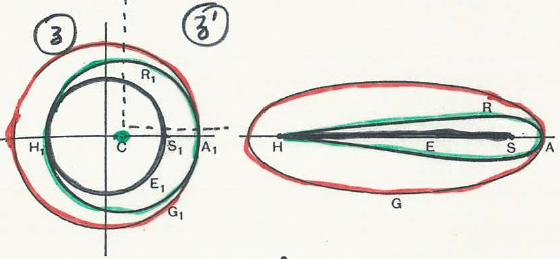
\includegraphics[scale=0.3]{ch2/31}
		\captionof{figure}{}
	\end{minipage}
	\begin{minipage}{0.45\textwidth}
		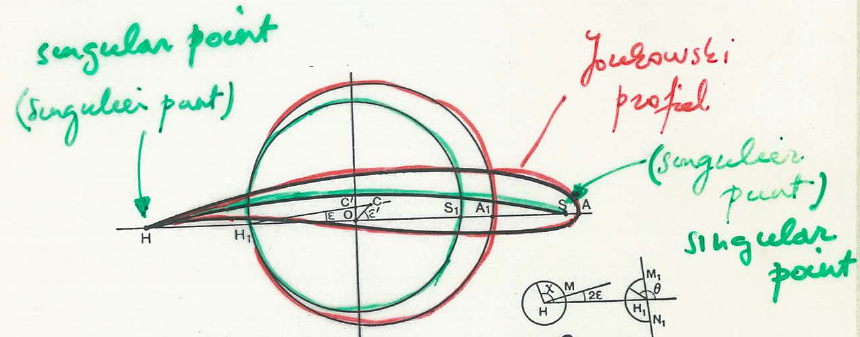
\includegraphics[scale=0.2]{ch2/32}
		\captionof{figure}{}
	\end{minipage}
\end{center}

Note that for the green circle in first figure, the complex potential becomes:

\begin{equation}
w = U\left( z-z_c + \frac{r^2}{z-z_c} \right)
\end{equation}

As last remark, let's remind that we had singularities in the second example. These points corresponds here to $H_1$ and $S_1$. The mapping of $H_1$ is always H the trailing edge, the velocity is there infinitely large. This was the discussion we've previously done with the stagnation point that has to move on the trailing edge otherwise $v = \infty$ because of the sharp edge. We can solve this by adding a vortex. This methods gives a limited amount of airfoils.

%-----------------------------------------------------------------------------------------------------------------
%-----------------------------------------------------------------------------------------------------------------
%-----------------------------------------------------------------------------------------------------------------

\section{Computation of inviscid irrotational flow around a thin airfoil based on a
	continuous distribution of vortices}
\subsection{Explain what is a free vortex}

A free vortex is an irrotationnal vortex where the flow velocity u is inversely proportional to the distance r.
\begin{wrapfigure}[5]{l}{3cm}
	\vspace{-5mm}
	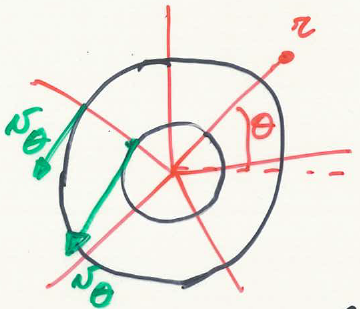
\includegraphics[scale=0.23]{ch2/26}
	\captionof{figure}{}
\end{wrapfigure}

Streamlines are circles oriented in negative rotational motion around z-axis (z entering in the sheet) so clockwise. We can compute the velocity field by deriving among z and we find that: 

\begin{equation}
u = \frac{\Gamma \sin \theta}{2 \pi r} \qquad v = -\frac{\Gamma \cos \theta}{2\pi r}
\end{equation}

Let's specify that $v_\theta = \frac{1}{r} \frac{\D \phi}{\D \theta} = -\frac{\Gamma}{2 \pi r}$, and that we have a vortex singularity in the center because $\Gamma = 0. \infty$.

\subsection{Explain what is a continuous distribution of free vortices on a line}

A way to represent thin airfoils is to use only their camberline and to retrieve the flow using an infinite line of free vorticies (or sources). A infinite line of vorticies thus represents an infinite thin airfoil.

\subsection{Explain principle of the method of free vortex distribution applied thin airfoils,
	limitations and hypotheses}

We will suppose infinitely thin airfoil and small angle of attack, so that the airfoil is represented by the camber line. This means also small camber about 2-3\% of the chord and $\alpha <8\%$. We can try to retrieve the flow by superposition principle by using infinite number of elementary sources or elementary vorticies. The potential function for the sources is:

\begin{equation}
\phi = \frac{\Lambda}{2\pi} \ln r \qquad d\phi = \frac{d\Lambda}{2\pi} \ln r
\end{equation}		

We then describe the source distribution by the source intensity $\lambda = \frac{d\Lambda}{ds}$ on a part $ds$ of the wing so that the last equation becomes:

\begin{equation}
d\phi = \frac{\lambda}{2\pi} \ln r\, ds.
\end{equation}

We will use the second method presented now which is using the vorticies: 

\begin{equation}
\phi = -\frac{\Gamma}{2\pi} \theta \qquad \vec{v} = \nabla \phi = \underbrace{\frac{\D \phi}{\D r} \vec{1}_r}_{= v_r = 0} + \underbrace{\frac{1}{r} \frac{\D \phi}{\D \theta} \vec{1} _\theta}_{= v_\theta} \qquad \Rightarrow v_\theta = -\frac{\Gamma }{2\pi} \frac{1}{r}.
\end{equation}

In the same way as the other we can define a \textbf{vortex intensity} to characterize the vortex distribution on a part ds $\gamma = \frac{d\Gamma}{ds}$, the derivative of $\phi$ and the elementary velocity are then: 

\begin{equation}
d\phi = -\frac{\gamma}{2\pi} \theta \, ds \qquad dv_\theta = -\frac{\gamma ds}{2\pi r}.
\end{equation}

The aim now is to make that infinitely thin airfoil a streamline. We assume because of superposition that the flow is a uniform flow $\vec{U}_\infty$, that we have an angle of attack $\alpha$. Because of the vorticies, we have a velocity perturbation $\vec{v}$ such that the total velocity is: 

\begin{equation}
\vec{V}_\infty = \vec{U}_\infty + \vec{v}.
\end{equation}

\subsection{Establish the integral equation which allows to compute the vortex
	distribution for a given profile}

\begin{wrapfigure}[9]{l}{8.5cm}
	\vspace{-5mm}
	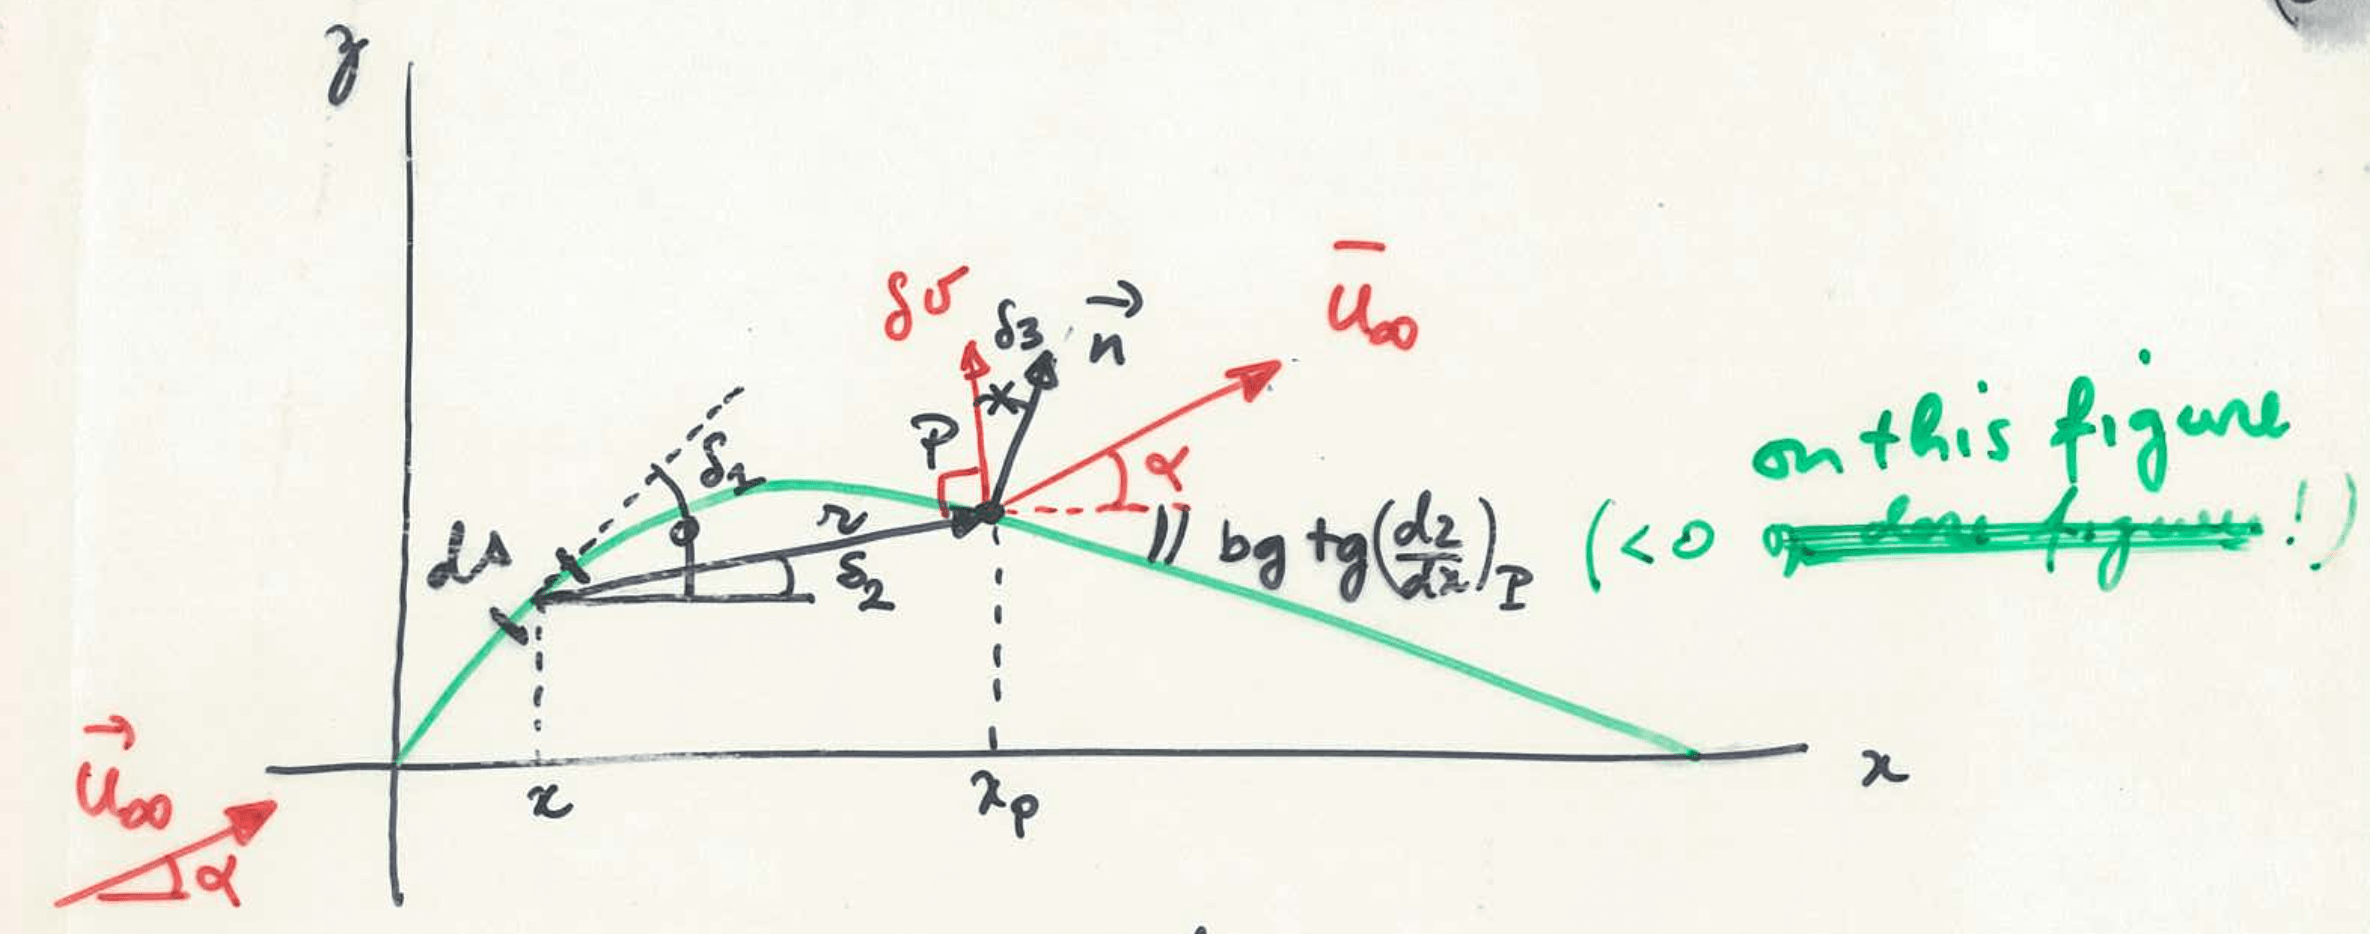
\includegraphics[scale=0.1]{ch2/33}
	\captionof{figure}{}
\end{wrapfigure}
We must now choose $\gamma$ such that $\vec{V}$ is tangential to the airfoil everywhere (we want the camber line to be a streamline). In other words, $\forall P$ the normal component of the velocity should be null $V_{nP} = U_{\infty _{nP}} + v_{nP} = 0$. Let's determine these components by projection. First, for $U_{\infty _{nP}}$ we can remark the sum of angle $\alpha$ and the camber line slope $\tan \beta =  \left(-\frac{dz}{dx}\right)_p \Rightarrow \beta = -\arctan \left(\frac{dz}{dx}\right)_p$, the projection is (camber line: $z = f(x)$):

\begin{equation}
U_{\infty _{nP}} = U_\infty \sin \left[ \alpha - \arctan \left(\frac{dz}{dx} \right)_P \right].
\label{eq:2.54}
\end{equation}	 

Now for $v_{np}$, we consider an elementary vortex on a point $x$ on the airfoil that creates an elementary perturbation $\delta v_n$ on point P. This velocity direction is $\theta$ in a $(r,\theta)$ axis with origin at x, so perpendicular to r on the figure. If the angle with the normal is $\delta _3$, the projection will be:

\begin{equation}
\delta v_n = -\frac{\gamma (x) ds}{2\pi r} \cos \delta _3 .
\end{equation}

Now we have infinite number of contribution of the infinite vorticies, as $\gamma , r$ and $\delta _3$ depend on position $P$, we have to integrate over the whole airfoil:

\begin{equation}
v_n = - \frac{1}{2\pi }\int _0 ^c \frac{\gamma (x) ds}{r} \cos \delta _3
\end{equation}

where $c$ is the chord length. We can express both $r$ and $ds$ in function of x as: 

\begin{equation}
r = \frac{x_P - x}{\cos \delta _2} \qquad ds = \frac{dx}{\cos \delta _1}
\end{equation}

which gives 
\begin{equation}
v_n = - \frac{1}{2\pi }\int _0 ^c \frac{\gamma (x) dx}{x_P - x} \frac{\cos \delta _2}{\cos \delta _1}\cos \delta _3. 
\end{equation}

We are able to reconsider the condition \eqref{eq:2.54} by replacing our results: 

\begin{center}
	\theor{
		\begin{equation}
		\frac{1}{2\pi }\int _0 ^c \frac{\gamma (x) dx}{x_P - x} \frac{\cos \delta _2}{\cos \delta _1}\cos \delta _3 =  U_\infty \sin \left[ \alpha - \arctan \left(\frac{dz}{dx} \right)_P \right].
		\end{equation}
	}
\end{center}

This is a relatively complicated equation, we can simplify it by \textbf{assuming a small camber} (in practice 2\% of the chord), which allows to say that $\delta _1 \approx \delta _2 \approx \delta _3 \approx 0$ and $\arctan \left( \frac{dz}{dx}\right) _P = \left( \frac{dz}{dx}\right) _P$. By considering $\alpha$ small, $\sin \alpha \approx \alpha$:

\begin{equation}
\frac{1}{2\pi} \int _0 ^c \frac{\gamma (x)\, dx}{x_P - x} = U_{\infty}\left[ \alpha -  \left(\frac{dz}{dx} \right)_P \right].
\end{equation}

We will introduce a new variable $\theta$, considering $x = \frac{1}{2}c (1-\cos \theta)$ and $dx = \frac{1}{2}c \sin \theta\, d\theta$: 

\begin{equation}
\frac{1}{2\pi} \int _0 ^{\pi} \frac{\gamma (\theta)\sin \theta \, d\theta}{\cos \theta - \cos \theta _P} = U_{\infty}\left[ \alpha -  \left(\frac{dz}{dx} \right)_P \right].
\label{eq:2.61}
\end{equation}

\subsection{Show how to solve this equation using a spectral method, i.e. by expressing
	the vortex distribution as a truncated Fourier series}


Let's express $\gamma (\theta )$ in series: 

\begin{equation}
\gamma (\theta ) = 2U_\infty \left(A_0 \coth \frac{\theta }{2} + \sum _{n=1}^\infty) A_n \sin (n\theta)\right).
\end{equation}

This is in fact a solution of the last equation. 

Now we can replace this definition on the previous equation, knowing that $\coth (\theta /2) \sin \theta = 1+\cos \theta$ and writing $\theta _P = \theta '$, we get:

\begin{equation}
\frac{1}{2\pi} \int _0 ^{\pi} \frac{\gamma (\theta)\sin \theta \, d\theta}{\cos \theta - \cos \theta _P}  = \frac{U_\infty}{\pi} \left[ \int _0 ^{\pi} \frac{A_0 (1+\cos \theta ) \, d\theta}{\cos \theta - \cos \theta '} + \sum _n A_n \int _0 ^{\pi}  \frac{\sin (n\theta)\sin \theta \, d\theta}{\cos \theta - \cos \theta '}  \right]
\end{equation}

By using the equality here and the \textbf{Glauert integral}:

\begin{equation}
\sin (n\theta ) \sin \theta = - \frac{1}{2} [\cos [(n+1)\theta] - \cos [(n-1)\theta]] \qquad \int _0 ^\pi \frac{\cos (n\theta)\, d\theta}{\cos \theta - \cos \theta '} = \pi \frac{sin(n\theta ')}{sin \theta '}
\end{equation}

The integral becomes: 

\begin{equation}
\frac{U_\infty}{\pi} \left[ A_0.0 + A_0. \pi - \frac{\pi}{2} \sum _n A_n \frac{\sin [(n+1)\theta '] - \sin [(n-1)\theta ']}{\sin \theta '} \right] = U_\infty \left[ A_0 - \sum _n A_n \cos (n\theta ') \right]
\end{equation}

where we used the Simpson equation. The \eqref{eq:2.61} becomes: 

\begin{center}
	\theor{
		\begin{equation}
		A_0 - \sum _n A_n \cos (n\theta ') = \alpha - \left( \frac{dz}{dx} \right)'
		\end{equation}
	}
\end{center}

This equation must be valid $\forall P$ on the airfoil. To find the coefficients $A_i$, let's integrate first this for $0\leq \theta ' \leq \pi$ in order to compute $A_0$: 

\begin{equation}
A_0\pi - \cancel{\sum _n A_n \int _0 ^\pi \cos (n\theta ')d\theta '} = \alpha\pi - \int _0 ^\pi \frac{dz}{dx}d\theta\qquad \Rightarrow A_0 = \alpha - \frac{1}{\pi} \int _0^\pi \frac{dz}{dx}\, d\theta.
\end{equation}

For the $A_n$, we multiply the same equation by $\cos (m\theta ')$ before integrating (we will drop the '). Let's see that $\int _0 ^\pi \cos (n\theta)\cos (m\theta) d\theta = 0$ if $ m \neq n $ and $= \pi /2$ if $n = m$. We finally get:

\begin{equation}
A_n = \frac{2}{\pi} \int _0 ^\pi \frac{dz}{dx} \cos (m\theta) \, d\theta .
\end{equation}

We can note that for $A_n$ only the camber plays a role, the angle of attack does not appear. Only $A_0$ is influenced by $\alpha$. We are now able to compute any vorticity distribution $\gamma (\theta)$, for example for a flat plate $A_n = 0$ and $A_0 = \alpha$. 

\subsection{How is the Kutta-Youkowski condition imposed (allowing to compute the lift)}

The above respects the Kutta condition that states that there is no vortex allowed on the trailing edge. Indeed, $\gamma (\pi) = 0$  which means no contribution by vortex. We can also state that at the leading edge, the stagnation point is in the pressure side at the front. Indeed, for $\theta = 0$, $\coth \theta = \infty = \gamma (\pi )$ which means that we have a singularity at the TE and that the velocity is infinite due to the turning on the LE. 

\subsection{Starting from the expressions for the Fourier coefficients, compute the
	circulation and lift coefficient as a function of angle of attack, explain the
	result}

\subsubsection{Calculation of the total circulation}

To get $\Gamma$ we only have to compute the integral over the whole airfoil:

\begin{equation}
\begin{aligned}
\Gamma &= \int _0 ^c \gamma (x) \, dx = \frac{1}{2} c \int _0 ^c \gamma (\theta ) \sin \theta \, d\theta \\
& = \frac{1}{2} c \left[ 2U_\infty \int _0 ^\pi A_0 (1+\cos\theta) \, d\theta + 2U_\infty \sum _{n=1}^\infty \int _0^\pi A_n \sin (n\theta)\sin \theta \, d\theta  \right] \\
&= U_\infty  c \left[  A_0 \pi  + 2U_\infty + \int _0^\pi \sin ^2(\theta) \, d\theta - \frac{1}{2} \sum _{n=2}^\infty \cancel{\int _0^\pi A_n \cos [(n+1)\theta - \cos (n-1)\theta ] \, d\theta } \right] \\
&= U_\infty c [A_0 \pi + A_1 \pi /2].
\end{aligned}
\end{equation}

We see that the circulation only depends on two coefficients. 

\subsubsection{Calculation of the lift coefficient}
We can now compute the lift using the kutta formula $L = \rho _\infty U_\infty \Gamma$. We are interested in the $c_l$ and not the lift itself. In 2D we have to divide by the chord so: 

\begin{equation}
c_l = \frac{L}{\frac{1}{2} \rho _\infty U_\infty ^2 C} = \frac{2\Gamma}{U_\infty c} = \pi (2A_0 + A_1)
\label{eq:2.70}
\end{equation}

We can now replace by definition of the coefficients: 

\begin{equation}
c_l = 2\pi\left(\alpha - \underbrace{\frac{1}{\pi} \int _0^\pi \frac{dz}{dx} (1-\cos \theta)\, d\theta}_{\alpha _0} \right) = 2\pi (\alpha - \alpha _0)
\label{eq:2.71}
\end{equation}

where $\alpha _0$ is the \textbf{zero lift angle of attack}. We see that we have a linear relation with respect to $\alpha$. We have the theoretical model the same for every profile, only $\alpha _0$ changes with the profile. Remark that the lift is also the integral of the pressure on the lower and upper side:

\begin{equation}
L = \int _0 ^c (p_l - p_u) \, dx = \rho _\infty U_\infty \int _0 ^c \gamma \, dx \qquad \Rightarrow p_l - p_u = \rho _\infty U_\infty \gamma (x).
\end{equation}

\subsection{Starting from the expression for the momentum coefficient at the leading
	edge $c_m$(LE), show that it’s a linear function of the lift coefficient $c_l$}


\begin{wrapfigure}[5]{l}{4.5cm}
	\vspace{-5mm}
	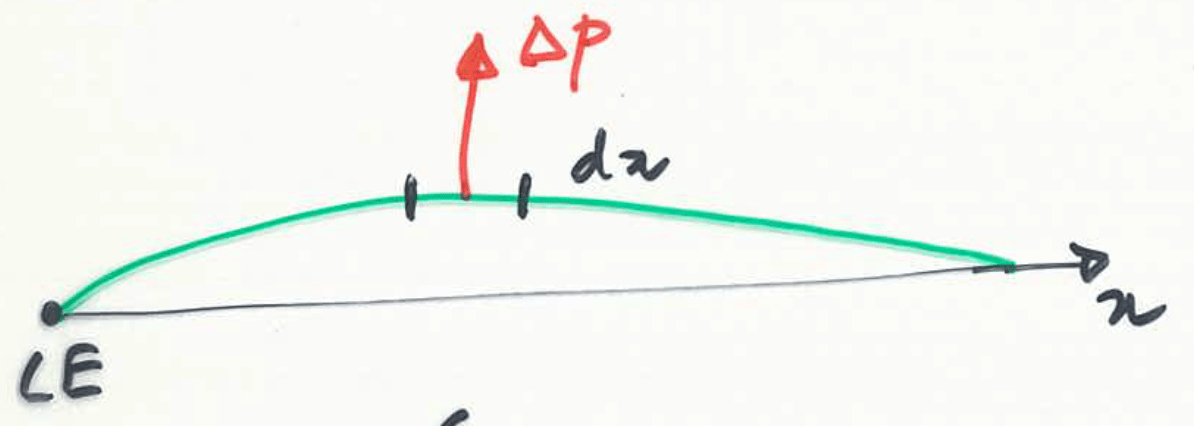
\includegraphics[scale=0.1]{ch2/34}
	\captionof{figure}{}
\end{wrapfigure}
The contribution of the elementary parts of the airfoil gives:

\begin{equation}
\begin{aligned}
&dM_{LE} = - (\Delta p \, dx) x \\ 
\Rightarrow &M_{LE} = -\int _0 ^c \Delta p x \, dx = - \rho _\infty U_\infty \int _0^c \gamma x \, dx
\end{aligned}
\end{equation}

After some manipulations (not detailed):

\begin{equation}
c_{m_{LE}} = \frac{M_{LE}}{\frac{1}{2}\rho _\infty U_\infty ^2 c^2} = - \frac{\pi}{4} (2A_0 + 2A_1 - A_2) = -\frac{1}{4} c_l - \frac{\pi}{4} (A_1 - A_2)
\end{equation}

where we used \eqref{eq:2.70} for the last expression.

\subsection{Compute the location of the aerodynamic center AC and the momentum
	coefficient in the aerodynamic center}

\begin{wrapfigure}[6]{l}{4.5cm}
	\vspace{-5mm}
	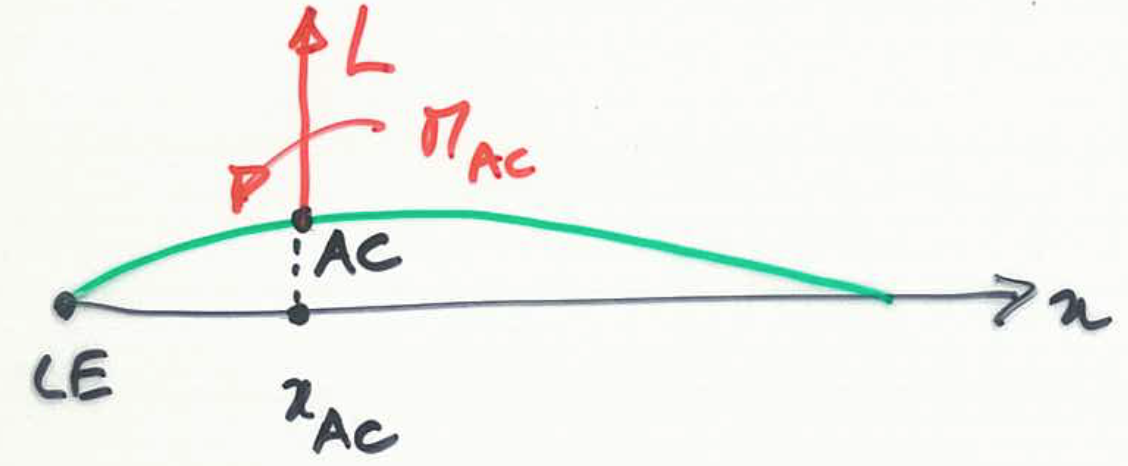
\includegraphics[scale=0.1]{ch2/35}
	\captionof{figure}{}
\end{wrapfigure}
The moment on the LE is related to the moment anywhere:

\begin{equation}
M_{LE} = M_{ac} - x_{ac} L \qquad \Rightarrow c_{m_{LE}} =c_{m_{ac}} - \frac{x_{ac}}{c}c_{l} 
\end{equation}

By using the last result of the previous section, we get: 

\begin{equation}
c_{m_{ac}} = \left( \frac{x_{ac}}{c} - \frac{1}{4} \right) c_l - \frac{\pi}{4} (A_1 -A_2).
\end{equation}

We see that, for this relation to be independent of the angle of attack, we must have $x_{ac} = \frac{c}{4}$ so that: 

\begin{equation}
c_{m_{ac}} = \frac{\pi}{4} (A_2 - A_1).
\label{eq:2.77}
\end{equation}

Remark that for symmetrical wings $\frac{dz}{dx} = 0 \Rightarrow A_1 = A_2 = 0 \Rightarrow c_{m_{ac}} = 0$. 

\subsection{Compute the location of the center of pressure}

The formula used in the previous section is valid, we replace ac by cp, and since the moment should be null at this point:

\begin{equation}
c_{m_{cp}} = c_{m_{LE}} + \frac{x_{cp}}{c} c_l = 0 \qquad \Rightarrow \frac{x_{cp}}{c} = \frac{1}{4} + \frac{\frac{\pi}{4}(A_1-A_2)}{c_l} = \frac{1}{4} - \frac{c_{m_{ac}}}{c_l}.
\end{equation}

Some remarks: 

\begin{itemize}
	\item[•] the center of pressure is not fixed and varies with the lift
	\item[•] at 0 lift, $x_{cp}\rightarrow \infty$ (for symmetric wing $x_{cp} = x_{ac} = c/4$ fixed)
	\item[•] cp always downstream to ac because $c_{m_{ac}}<0$.
\end{itemize}


%-----------------------------------------------------------------------------------------------------------------
%-----------------------------------------------------------------------------------------------------------------
%-----------------------------------------------------------------------------------------------------------------

\section{Computation of inviscid irrotational flow around a thin airfoil based on a
	continuous distribution of vortices}
\paragraph{Discuss the influence of a flap located at the trailing edge of the airfoil}
	According to the definition of the zero lift angle in \eqref{eq:2.71}, the effect of the shape becomes greater when $\theta \approx 180\degres$ (trailing edge). By making the zero lift angle more negative we can produce more lift before the critical angle of attack that decreases a bit.
	
		\begin{wrapfigure}[6]{r}{3.5cm}
		\vspace{-5mm}
		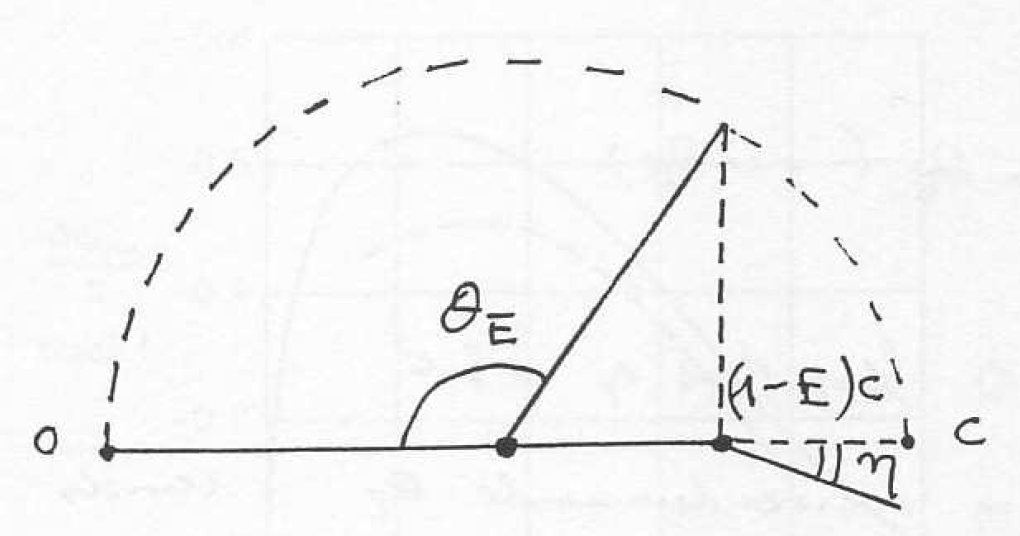
\includegraphics[scale=0.1]{ch2/37}
		\captionof{figure}{}
	\end{wrapfigure}
	The effect is evaluated by taking a flat plate as camber line with a deflection near the TE, starting at E\% of the chord and slope $\eta$. E in function of $\theta _E$ is: 
	
	\begin{equation}
	E = \frac{1}{2} (1+\cos \theta _E).
	\end{equation}	 
	
	In this case, $A_0$ and $A_n$ can be rewritten as:
	
	\begin{equation}
	\begin{aligned}
	&A_0 = \alpha - \frac{1}{\pi} \int _0 ^\pi \frac{dz}{dx} d\theta \approx \alpha - \frac{\eta}{\pi} (\pi - \theta _E) \\
	&A_n = \frac{2}{\pi} \int _0 ^\pi \frac{dz}{dx} \cos (n\theta )d\theta \approx -\frac{2\eta}{\pi} \frac{1}{n} \sin (n\theta _E)
	\end{aligned}
	\end{equation}
	
	such that the lift coefficient becomes: 
	
	\begin{equation}
	c_l = \pi (2A_0 + A_1) = \underbrace{2\pi \alpha}_{\mbox{without flaps}} \underbrace{- 2\eta (\pi - \theta _E + \sin \theta)}_{\Delta c_l > 0 \mbox{ since } \eta < 0}.
	\end{equation}
	
	This seams to be like $c_l = 2\pi (\alpha - \alpha _0)$ allowing the definition for the zero lift angle: 
	
	\begin{equation}
	\alpha _0 = \frac{\eta}{\pi} (\pi - \theta _E + \sin \theta)
	\end{equation}
	
	which indicates an increase (decrease since $\eta <0$) of $\alpha _0$ since it is null for the flat plate. For the moment at the ac \eqref{eq:2.77}
	
	\begin{equation}
	\Delta c_{m_{ac}} = \frac{\eta }{2} \sin \theta _E (1- \cos \theta _E)
	\end{equation}
	
	which also indicates a decrease in the momentum which is 0 for the symmetric wing.
\paragraph{Determine the effect of the flap on:}
\begin{description}
	\item[the lift curve:] from the above, we see that lift goes up with flaps
	\item[the zero lift angle of attack:] It is increased, see above
	\item[the moment at the aerodynamic center:] It decreases.
\end{description}


%-----------------------------------------------------------------------------------------------------------------
%-----------------------------------------------------------------------------------------------------------------
%-----------------------------------------------------------------------------------------------------------------

\section{3D wing theory}

\subsection{Explain mean chord, span, aspect ratio, taper, sweep of wing}
\begin{center}
	\begin{minipage}{0.4\textwidth}
		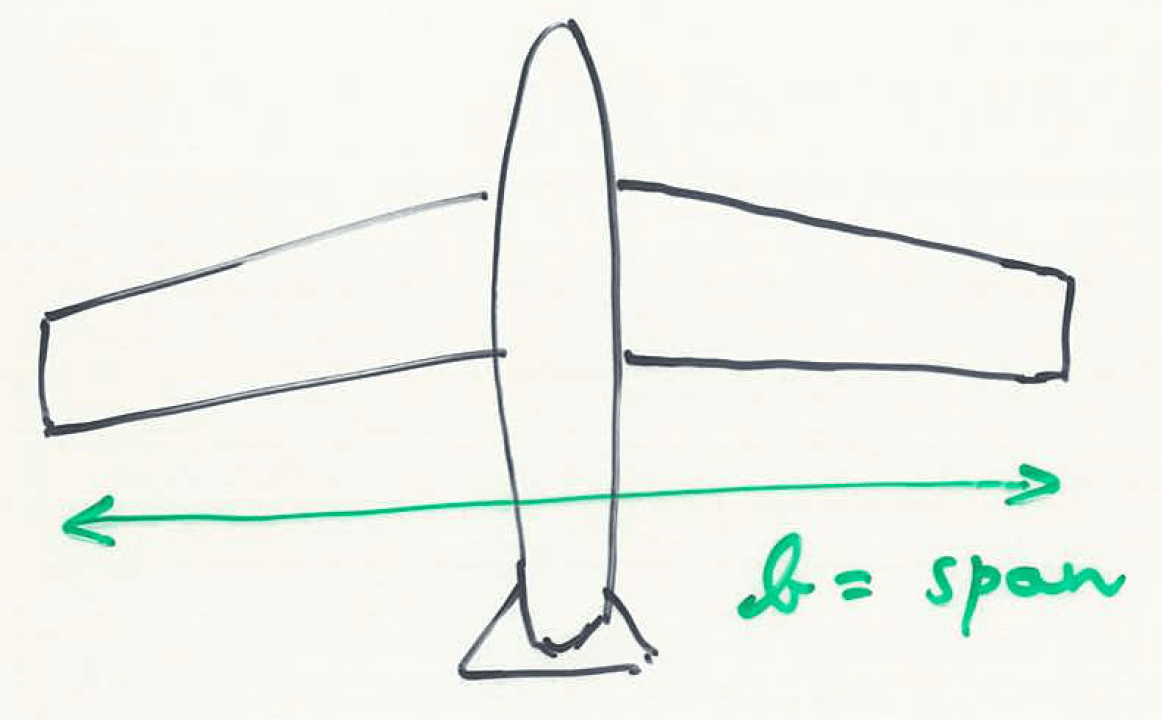
\includegraphics[scale=0.1]{ch3/1}
		\captionof{figure}{}	
	\end{minipage}
	\begin{minipage}{0.3\textwidth}
		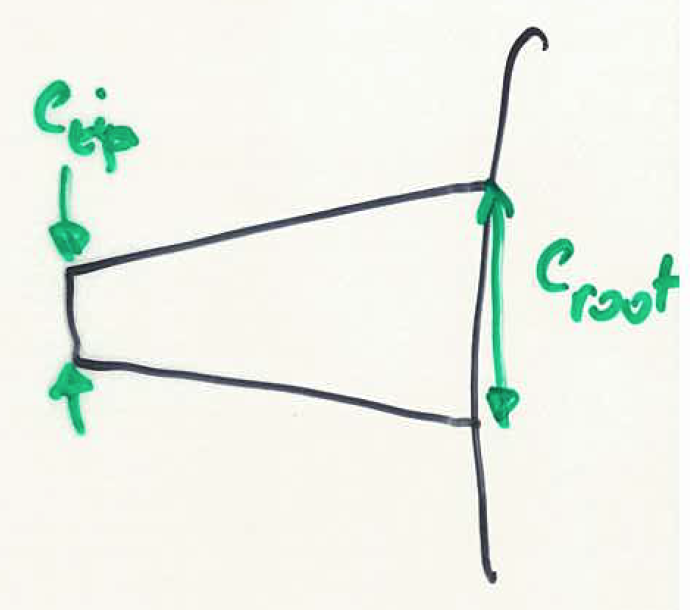
\includegraphics[scale=0.15]{ch3/2}
		\captionof{figure}{}	
	\end{minipage}
\end{center}
The \textbf{span} is the total distance between the tips of the wings, plane body included. It is a straight line.\\
The \textbf{mean chord} is defined by dividing the wing area by the span. This is used to avoid having a chord that varies for calculations.\\
The \textbf{aspect ratio} is the span divided  by the mean chord, or the span squared divided by the wing surface. Higher aspect ration means higher lift to drag ratio.\\
\textbf{Tapered wings} are wing that have a bigger chord near the body. The \textbf{taper ratio} is defined by $\frac{c_{tip}}{c_{root}}$\\
\textbf{Swept wings} are wings that are (at least partially) not $\perp$ to the flow. This is to delay shock wave formation. The sweep is the angle of the leading and/or trailing edge compared to the $\perp$ to the flow.

\subsection{Explain downwash effect, downwash angle, effective angle of attack, total and
	induced drag}
\wrapfig{7}{l}{6.5}{0.1}{ch3/3}{fig:3.3}
Finite span $\Rightarrow$the pressure on both side must be equal at the end of the span. This means that the pressure on the upper side must increase when going to the tip, and decrease on the lower side. This creates a pressure gradient between the root and the tip. This gradient will push the streamlines on the upper side towards the fuselage and towards the tip on the lower side. 

\begin{center}
	\begin{minipage}{0.4\textwidth}
		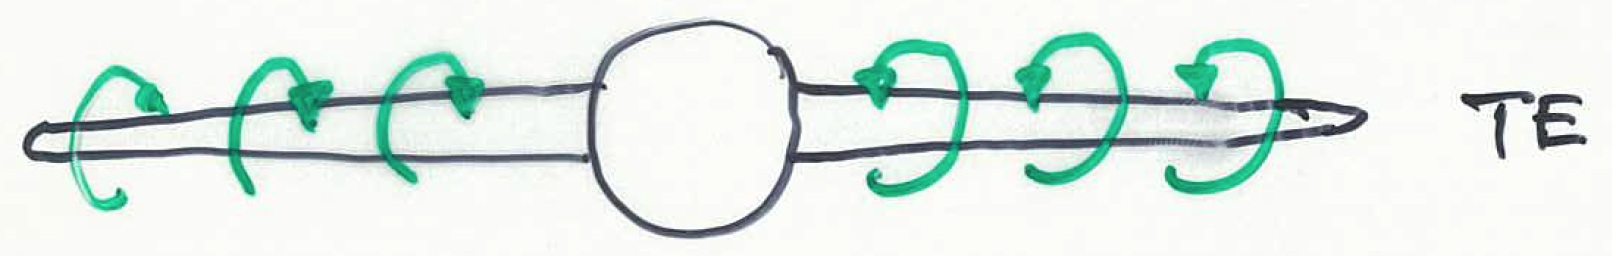
\includegraphics[scale=0.1]{ch3/4}
		\captionof{figure}{}	
		\label{fig:3.4}
	\end{minipage}
	\begin{minipage}{0.4\textwidth}
		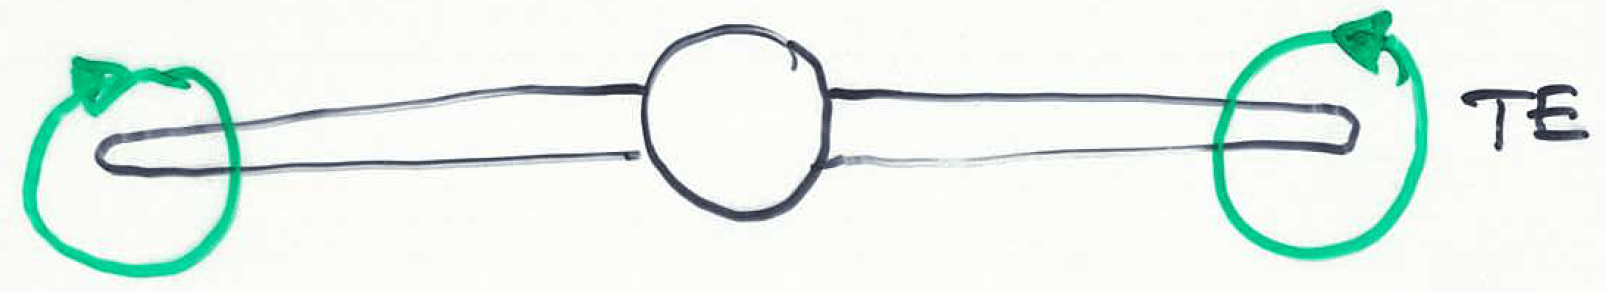
\includegraphics[scale=0.1]{ch3/5}
		\captionof{figure}{}	
		\label{fig:3.5}
	\end{minipage}
\end{center}

Looking from downstream, this discontinuity in velocity induces an infinite series of infinitely small vortices, clockwise on the left and anti clockwise on the right wing (\autoref{fig:3.4}), resulting in 2 discrete vortices at the tip, the s\textbf{wong-tip vortices or trailing vortices} (\autoref{fig:3.5}). 

\wrapfig{7}{l}{6.5}{0.08}{ch3/6}{fig:3.6}
These vortices induce a \textbf{downward velocity component, the downwash} $\vec{w}$. This component superposes on the incoming flow and changes the angle of attack (\autoref{fig:3.6}). The angle of change is the \textbf{downwash angle}, or induced angle of attack and we compute the \textbf{effective angle of attack} $\alpha _{eff} = \alpha - \epsilon$ where $\epsilon$ is the induced angle of attack.

The decrease of $\alpha$ means a decrease in liftas the new lift is perpendicular to the new flow, some oof it's force produces an \textbf{induced drag}.

The \textbf{total drag $C_D$} is computed as being the sum of the profil drag and the induced one. (in reality, we also have to take into account the parasite drags created by the fuselage, antennas,...)

\subsection{Starting from the given expression for the downwash angle, compute the induced
	drag force and the induced drag coefficient}

\begin{equation}
\alpha _{eff} = \alpha - \epsilon
\end{equation}

\textbf{induced drag}: 

\begin{equation}
D_i = L \sin \alpha _i \approx L\alpha _i \qquad with \qquad \alpha _i = \frac{C_L}{\pi e AR} 
\label{eq:3.2}
\end{equation}

\wrapfig{10}{r}{5.5}{0.1}{ch3/7}{fig:3.7}
where $e$ is the \textbf{span efficiency factor or Oswald's efficiency factor} $0.85<e<1$. We get the Drag coefficient:

\begin{equation}
C_{D_i} =  \frac{C_L^2}{\pi e AR} .
\end{equation}

\subsection{Explain the lift curve as a function of the angle of attack for a 3D wing, compare
	with the lift curve for a 2D profile}
The theoretical lift curve can be obtained based on the 2D wing as \autoref{fig:3.7}. We can see that the 3D wing lift for a certain $\alpha$ corresponds to the 2D lift for the effective angle of attack $\alpha - \epsilon$. The induced angle of attack decreases with lift, at $\alpha _0$ the two curve are on the same point. Algebraically the 2D and 3D curves can be noted:

\begin{equation}
c_l = m(\alpha - \alpha _0), \qquad C_L = m(\alpha - \epsilon - \alpha _0) = m^* (\alpha - \alpha _0)
\label{eq:3.4}
\end{equation}

where $m^*$ is the slope of the 3D lift. We can isolate this and find that:

\begin{equation}
m^* = m\left( 1 - \frac{\epsilon}{\alpha - \alpha _0} \right) = \frac{m}{1+\frac{m}{\pi e AR}} 
\end{equation}

where we used the definition \eqref{eq:3.2} and \eqref{eq:3.4} for the last result. We see that the slope is independent from $\alpha$. 

\subsection{Give the expression for the total drag coefficient as a function of $C_L$}

The total drag is the sum of the profile drag and the induced one:

\begin{equation}
C_D = C_{D_0} + kC_L^2 + C_{D_i} = C_{D_0} + C_L^2 \left( k + \frac{1}{\pi e AR}\right)
\end{equation}	 

where $k$ is generally small compared to the other. 

\wrapfig{8}{l}{5.5}{0.08}{ch3/8}{fig:3.8}
With these formulas we can plot the characteristics in 3D. We can note that the maximum lift does not change so more, but there is a strong decrease in the maximum glide ratio, $C_D$ increases with $C_L$ so $\alpha$. Finally we note an increase of the stall angle but in practice this is not as large as predicted. This means also that the maximum lift decreases slightly with decreasing AR. No significant difference for the moment. 

\wrapfig{5}{l}{5}{0.1}{ch3/9}{fig:3.9}
To avoid the adverse effect which is increasing induced drag. We can use high AR or add winglet on the tip, a kind of end plate that forces a vertical diffusion of the tip vortex, reducing drag. They have to be carefully designed to not increase the viscous drag. 

\subsection{Give the expression of the drag force D as a function of the velocity at infinity}

Let's compute the total drag using the coefficient definition:

\begin{equation}
\begin{aligned}
D &= C_D \frac{1}{2} \rho _\infty v_\infty ^2 S = C_{D_0} \frac{1}{2} \rho _\infty v_\infty ^2 S + \left(k +\frac{1}{\pi e AR} \right)\frac{L^2}{( \frac{1}{2} \rho _\infty v_\infty ^2 S)^2} \frac{1}{2} \rho _\infty v_\infty ^2 S \\
&= k_1 v_\infty ^2 + k_2 v_\infty^2.
\end{aligned}
\label{eq:3.7}
\end{equation}


%-----------------------------------------------------------------------------------------------------------------
%-----------------------------------------------------------------------------------------------------------------
%-----------------------------------------------------------------------------------------------------------------

\section{3D wing theory – Derivation of Prandtl lifting line method
	Give the basic ideas and the development of Prandtl’s lifting line theory}

\subsection{Velocity induced by a vortex filament}
\wrapfig{6}{l}{7}{0.12}{ch3/11}{fig:3.11}
The seen free vortex is characterized by circular streamlines around a certain point P. In this point the vorticity is concentrated such that the circulation around the contours that don't contain the point are null. If we consider several planes above each other containing a 2D free vortex, the point P form a line called \textbf{vortex line or vortex filament}. The circulation on each point of that line have the same circulation.

\wrapfig{6}{l}{6.5}{0.06}{ch3/13}{fig:3.13}
This line can be a random line with bending. Now if one places an infinite number of vortex lines besides each other, we get a \textbf{vortex sheet}.

The normal component of the velocity is continuous while the tangential one varies as $ \Delta v_t = \gamma $ with gamma given by the circulation around a vortex sheet.

\wrapfig{10}{l}{5}{0.1}{ch3/14}{fig:3.14}
Using Bio-Savart at point P:

\begin{equation}
\vec{v} = \frac{\Gamma }{4\pi}\int _{-\infty}^{+\infty} \frac{d\vec{l}\times r}{|r|^3}.
\end{equation}

We have: $d\vec{l} \times \vec{r} = Rdl \vec{1}_n$ , $\vec{v} = v \vec{1}_n$ (see figure). Let's define the length $l$ beginning from the piercing point on the surface until the $d\vec{l}$. We can graphically see that: 

\begin{equation}
l  = -R \coth \theta \Rightarrow dl = \frac{R}{\sin ^2\theta} d\theta, \qquad r = \frac{R}{\sin \theta} 
\end{equation}

Replacing all this we get:

\begin{equation}
v = \frac{\Gamma}{4\pi} \int _{0}^{\pi} \frac{R^2}{\sin^2 \theta } \frac{\sin ^3 \theta}{R^3} d\theta \qquad \Rightarrow v = \frac{\Gamma}{2\pi R}.
\end{equation}

This is the velocity distribution of the 2D free vortex.  

\subsection{Helmholtz theorems, Biot-Savart law}
\begin{center}
	\theor{\textbf{Helmholtz theorems}\\
		\begin{itemize}
			\item[•] Along a vortex line, the circulation must be constant.
			\item[•] A vortex line cannot finish in the flow but must continue to the edges of the flow or form a closed contour. 
		\end{itemize}
	}
\end{center}

\wrapfig{6}{r}{4}{0.1}{ch3/12}{fig:3.12}
This law gives the induced velocity in a certain point P cause by an elementary piece $d\vec{l}$ of the filament: 

\theor{
	\textbf{Law of Biot-Savart}
	\begin{equation}
	d\vec{v} = \frac{\Gamma }{4\pi} \frac{d\vec{l}\times r}{|r|^3}
	\end{equation}
}

\ \\ With analogy to electrical wire where we have a current intensity that induces a magnetic field on point P: $d\vec{B} = \frac{\mu I }{4\pi} \frac{d\vec{l}\times r}{|r|^3}$.
\subsection{Circulation around a vortex sheet}
 For the total circulation to be finite, the circulations must be infinitely small, but can vary from one line to the other. The circulation of the vortex sheet is calculated as:

\begin{equation}
\Gamma = \int _a ^b d\Gamma = \gamma \, ds
\end{equation}

\subsection{Downwash velocity induced by a single horseshoe vortex, why this model for a
	wing is not working}

\wrapfig{10}{l}{7}{0.08}{ch3/15}{fig:3.15}
The idea is to represent the 3D wing by means of vortex filaments. On the figure we have the \textbf{horseshoe vortex} where the x direction continues to infinity to satisfy the Helmholtz condition and the y direction extends from $-b/2$ to $b/2$ and represents the two wings. This last is the bound vortex and the one in x direction represents the tip vortices. The problem with the representation is that we have a constant circulation while we have seen that the lift decreases when going to the tips. 

\wrapfig{10}{r}{5}{0.1}{ch3/16}{fig:3.16}
Let's try to compute the downwash velocity on a point from the bound vortex. The law of Biot-Savart has 3 contributions: 

\begin{equation}
\vec{v} = \int _{-\infty} ^{-b/2} \dots + \int _{-b/2} ^{b/2} \dots + \int _{b/2}^{\infty}.
\end{equation}

The second integral vanishes as dl and r are parallel, the two others were computed at the previous section. Pay attention that we have to take half the contribution as the integral is not $-\infty,+\infty$:

\begin{equation}
\vec{v}(y) = \left(\frac{\Gamma}{4\pi R} + \frac{\Gamma}{4\pi R^*} \right) \vec{1}_n
\end{equation}

We can see that the velocity is infinity at the tips and minimum at the middle. This is clearly not the reality.

\subsection{Downwash velocity induced by a superposition of horseshoe vortices}
\begin{center}
	\begin{minipage}{0.4\textwidth}
		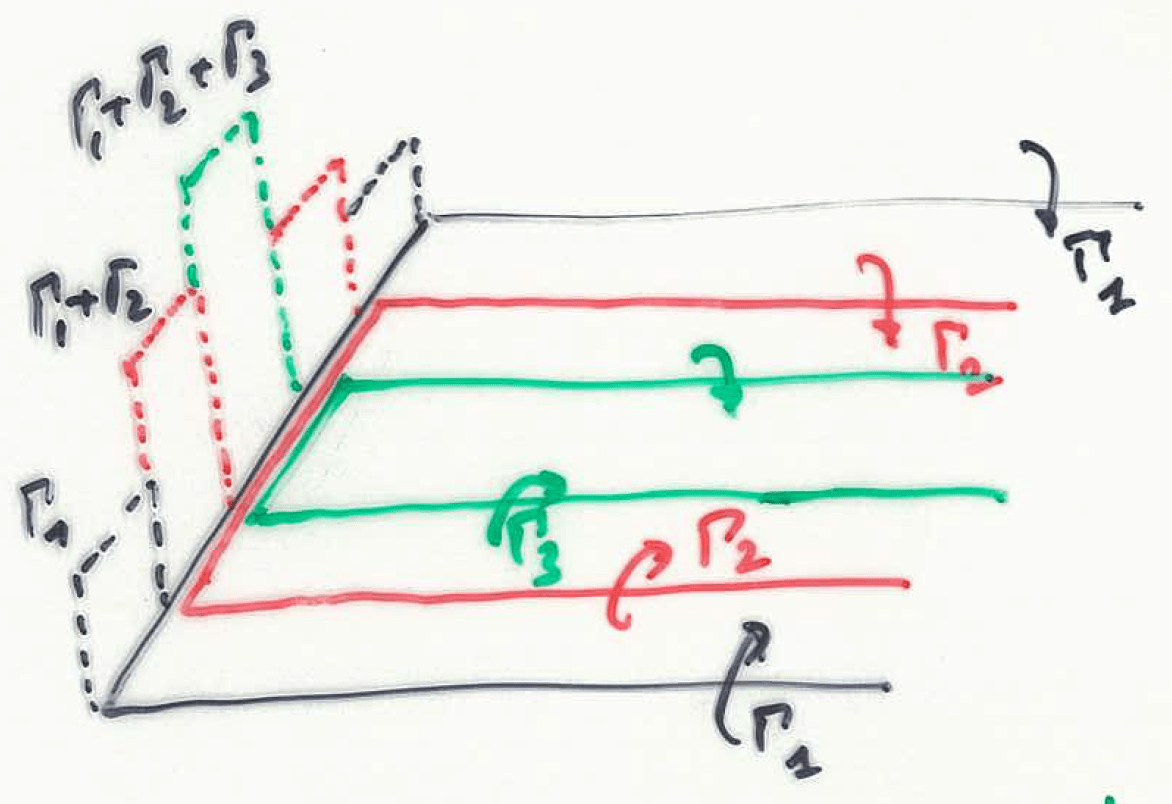
\includegraphics[scale=0.15]{ch3/17}
		\captionof{figure}{}	
		\label{fig:3.17}
	\end{minipage}
	\begin{minipage}{0.4\textwidth}
		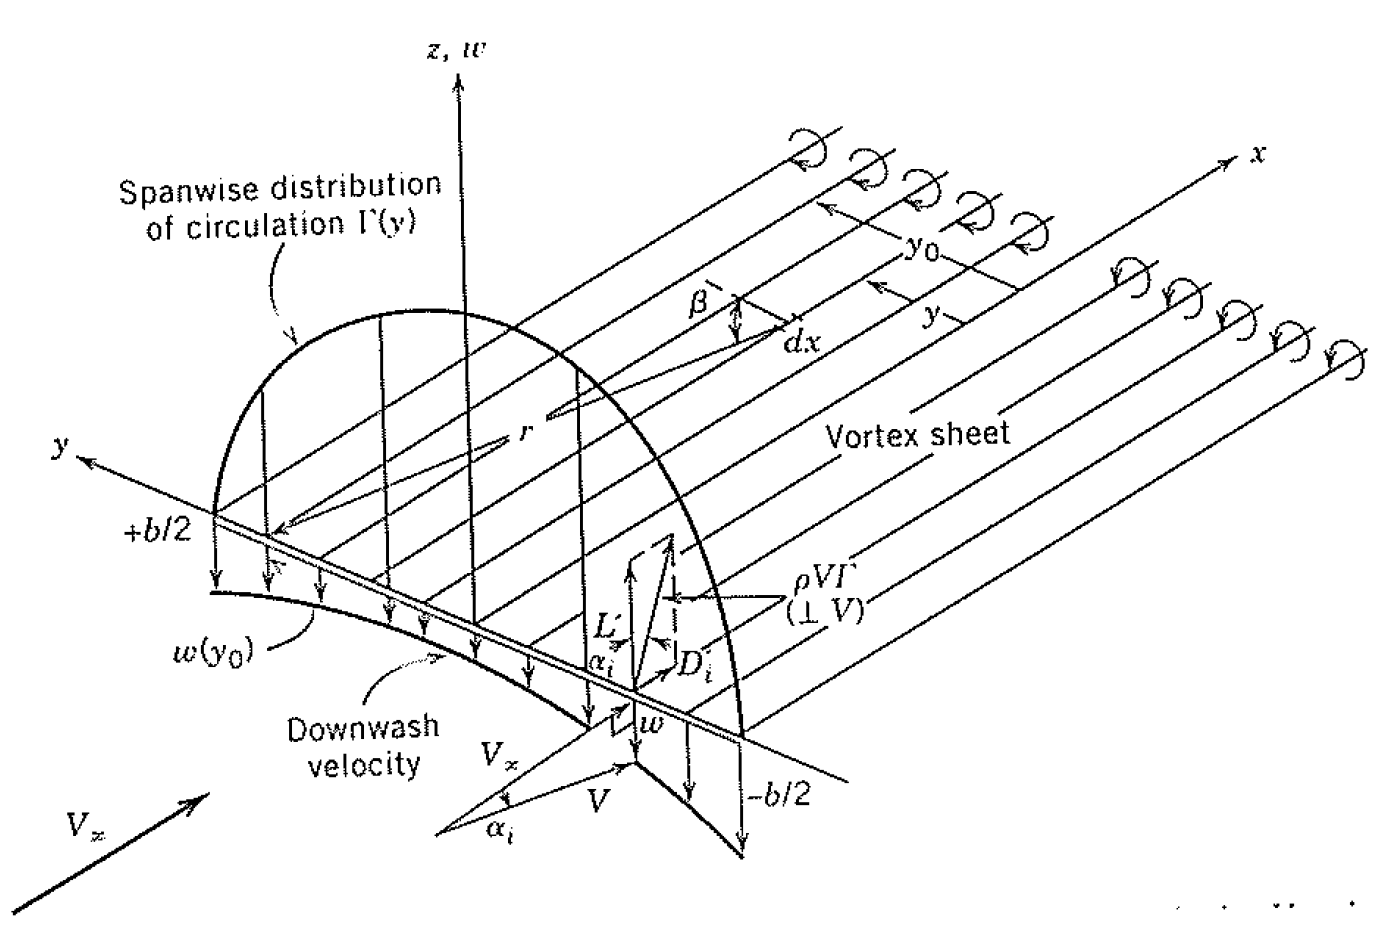
\includegraphics[scale=0.12]{ch3/18}
		\captionof{figure}{}	
		\label{fig:3.18}
	\end{minipage}
\end{center}

The solution is to superpose the horseshoes with bound vortices with different length (fig:\autoref{fig:3.17}). If now we let tend the number of superimposed horseshoe vortices to infinity, we will get a vortex sheet as represented on \autoref{fig:3.18}. The continuously varying circulation on the wing is no longer constant and this corresponds better with the reality. 

\wrapfig{10}{l}{5}{0.08}{ch3/19}{fig:3.19}
Consider this figure, we will try to compute the downwash velocity by considering a large but finite number of vortices of circulation $d \Gamma$ for each. We have 3 regions to consider with our basic formula:

\begin{itemize}
	\item[•] $y<0$: $d\vec{v}(y_0) =  \frac{d \Gamma}{4\pi (y_0-y)}\vec{1}_n$
	\item[•] $0<y<y_0$: $d\vec{v}(y_0) = \frac{d \Gamma}{4\pi (y_0-y)}\vec{1}_N = \frac{-d \Gamma}{4\pi (y_0-y)}\vec{1}_n$
	\item[•] $y_0<y$: $d\vec{v}(y_0) =  \frac{d \Gamma}{4\pi (y-y_0)}\vec{1}_n = \frac{-d \Gamma}{4\pi (y_0-y)}\vec{1}_n$  
\end{itemize}

We can see that the three formulas are the same if we take $\Gamma < 0$ for $y>0$. We can so write the total contribution and its extension to the infinite number of lines:

\begin{equation}
\vec{v} = \left[ \sum \frac{d\Gamma}{4\pi (y_0 - y)} \right] = \left[ \int _{-b/2}^{b/2} \frac{d\Gamma}{4\pi (y_0 - y)} \right]
\end{equation}


\subsection{Derivation of Prandtl’s fundamental equation of lifting line theory}
\wrapfig{10}{l}{5}{0.15}{ch3/20}{fig:3.20}
The induced angle of attack is then given by:

\begin{equation}
\tan \alpha _i \approx \alpha _i = \frac{v(y_0)}{v_\infty} = \frac{1}{4\pi v_\infty} \int _{-b/2} ^{b/2}\frac{d\Gamma}{y_0-y}.
\label{eq:3.18}
\end{equation}

Now let's denote $\alpha _{eff} = \alpha - \epsilon$. We know that the theory says $c_l = 2\pi (\alpha _{eff}(y_0)- \alpha _0(y_0))$, and using the definition of $c_l$ and the Kutta-Jukowski for $L(y_0)$ we get:

\begin{equation}
\begin{aligned}	
&c_l = \frac{L(y_0)}{\frac{1}{2}\rho_\infty v_\infty ^2 c(y_0)} = \frac{\rho _\infty v_\infty \Gamma (y_0)}{\frac{1}{2}\rho_\infty v_\infty ^2 c(y_0)} = \frac{\Gamma (y_0)}{\frac{1}{2}v_\infty ^2 c(y_0)} \\
&\Rightarrow \alpha _{eff} = \frac{\Gamma (y_0)}{\pi v_\infty c(y_0)} + \alpha _0(y_0)
\end{aligned}
\end{equation}

Combining all the result, we can compute the $\alpha$: 

\begin{center}
	\theor{
		\textbf{Fundamental equation of Prandtl's lifting line theory}
		\begin{equation}
		\alpha(y_0) = \frac{\Gamma (y_0)}{\pi v_\infty c(y_0)} + \alpha _0(y_0) + \frac{1}{4\pi v_\infty} \int _{-b/2}^{b/2} \frac{d\Gamma}{y_0 - y}. 
		\end{equation}		
	}
\end{center}

The only unknown in this equation is the circulation: several cases.
%-----------------------------------------------------------------------------------------------------------------
%-----------------------------------------------------------------------------------------------------------------
%-----------------------------------------------------------------------------------------------------------------

\section{3D wing theory: application of Prandtl lifting line theory for a wing with given
	circulation
	Starting from Prandtl’s fundamental equation of lifting line theory and the formula
	for the induced angle of attack:}
\begin{center}
	\theor{
		\textbf{Fundamental equation of Prandtl's lifting line theory}
		\begin{equation}
		\alpha(y_0) = \frac{\Gamma (y_0)}{\pi v_\infty c(y_0)} + \alpha _0(y_0) + \frac{1}{4\pi v_\infty} \int _{-b/2}^{b/2} \frac{d\Gamma}{y_0 - y}. 
		\end{equation}		
	}

\begin{equation}
\tan \alpha _i \approx \alpha _i = \frac{v(y_0)}{v_\infty} = \frac{1}{4\pi v_\infty} \int _{-b/2} ^{b/2}\frac{d\Gamma}{y_0-y}.
\label{eq:3.18}
\end{equation}


\end{center}

\subsection{Discuss the different terms of the equation}
$\Gamma$ is the circulation around the vortex sheet, $v_\infty$ the flow speed, $c(y_0)$ the point where we calculate the downwash,$y$ the position of a vortex wire. (see graphs above)

\subsection{Apply to a wing with a given circulation distribution: find lift and drag coefficients}

Idea is to solve the integral. The discussions below do it for more complicated case, so good luck!

\subsection{Apply to a wing with a given shape and unknown circulation distribution defined
	by a truncated Fourier series and compute the lift $C_L$ and the induced drag $C_{Di}$ coefficients}

Local and total lift by:

\begin{equation}
L'(y_0) = \rho _\infty v_\infty \Gamma (y_0) \qquad L = \int _{-b/2}^{b/2} L'(y)\, dy
\end{equation}

and the local and total induced drag: 

\begin{equation}
D'_i (y_0) = \Gamma (y_0) \epsilon (y_0) \qquad D_i = \int _{-b/2}^{b/2} D_i'(y)\, dy
\end{equation}

We assume a serie:

\begin{equation}
\Gamma = \sum _{n=1} ^N A_n \sin (n\theta).
\end{equation}

Substitution of this in the Prandtl's fundamental equation gives:

\begin{equation}
\alpha (\theta _0) = \frac{1}{\pi v_\infty c(\theta _0)} \sum _n A_n \sin (n\theta_0) + \alpha_0(\theta _0) + \frac{1}{2\pi v_\infty b} \sum _n A_n n \int ^0_\pi \frac{\cos (n\theta)d\theta}{\cos \theta _0 - \cos \theta}
\label{eq:3.32}
\end{equation}

$\rightarrow$ Glauert integral. We can find a solution by considering N equations for N points distributed along the span.

By integration of the local lift and definition of $C_L$ and $C_D$:
\begin{equation}
C_L = \frac{1}{\frac{1}{2}v_\infty S} \int _{-b/2}^{b/2} \Gamma (y) \, dy = \frac{b}{u_\infty S} \sum _n \int _0 ^\pi A_n \sin (n\theta) \sin \theta \, d\theta = \frac{\pi b A_1}{2Sv_\infty}. 
\end{equation}

\begin{equation}
C_{D_i} = \frac{1}{\frac{1}{2} v_\infty S} \int _{-b/2} ^{b/2} \Gamma (y)\alpha _i \, dy. 
\end{equation}

Using \eqref{eq:3.18}, we can express $\alpha _i (\theta _0)$ as:

\begin{equation}
\alpha _i (\theta _0) = \frac{1}{2\pi v_\infty b} \int ^{0}_{\pi} \frac{\frac{d\Gamma }{d\theta}}{\cos \theta _0 - \cos \theta} \, d\theta = \frac{1}{2\sin \theta _0 v_\infty b} \sum _n A_n n \sin (n \theta _0)
\end{equation}

which gives:

\begin{equation}
C_{D_i} = \frac{1}{2v_\infty ^2 S} \int _0 ^\pi \sum _n \sum _k A_n A_k \sin (n\theta) \sin (k\theta) \, d\theta = \frac{\pi}{4v_\infty ^2 S} \sum _n A_n ^2 n
\end{equation}

and using the lift coefficient:

\begin{equation}
C_{D_i} = \frac{C_L^2}{\pi AR}  \left(1+\sum _{n=2} n \left(\frac{A_n}{A_1}\right)^2 \right) \qquad \Rightarrow e = \frac{1}{1+\sum _{n=2} n \left(\frac{A_n}{A_1}\right)^2} = \frac{1}{1+\delta}
\end{equation}

where $\delta $ is the \textbf{induced drag factor}, since it is always positive, $e<1$. 

\subsection{Apply to a tapered wing}
\begin{center}
	\begin{minipage}{0.4\textwidth}
		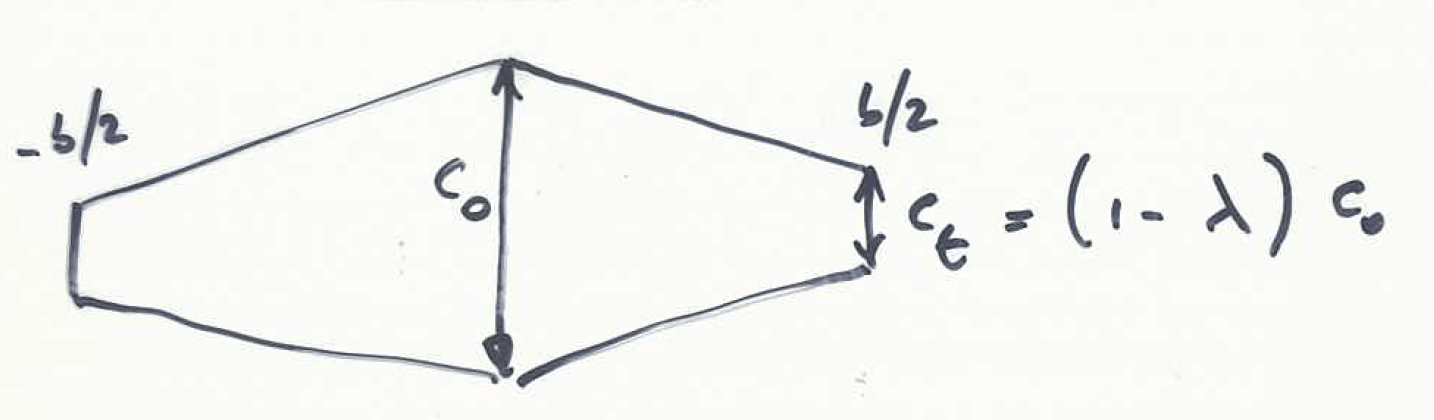
\includegraphics[scale=0.05]{ch3/21}
		\captionof{figure}{}	
		\label{fig:3.21}
	\end{minipage}
	\begin{minipage}{0.22\textwidth}
		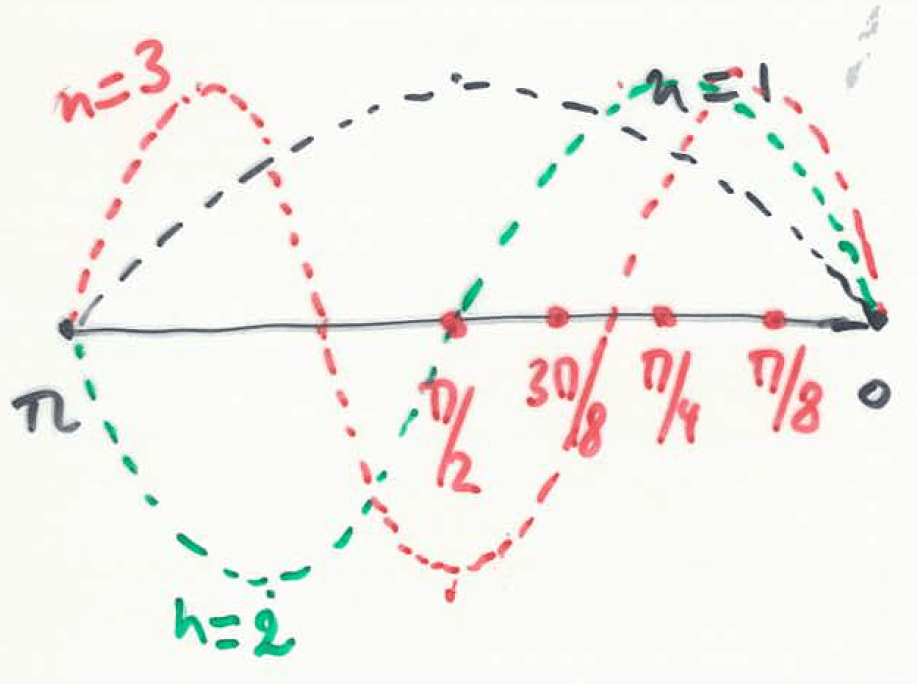
\includegraphics[scale=0.02]{ch3/22}
		\captionof{figure}{}	
		\label{fig:3.22}
	\end{minipage}
\end{center}

Same 2D profile along the span and no twist. Because of the symmetry, it is obvious that the pair n in the series will have no contribution. Let's go until 7:

\begin{equation}
\Gamma = A_1\sin \theta + A_3\sin 3\theta + A_5\sin 5\theta + A_7\sin 7\theta.
\end{equation}

To determine the coefficient we have to apply \eqref{eq:3.32} to 4 points. Let's take half the span because of symmetry: $\theta = \pi /8, \pi /4, 3\pi /8, \pi /2$. Since the 2D profile is constant, $\alpha _0$ is independent of $\theta$, same for $\alpha$ since there are no twist. 

\begin{center}
	\begin{minipage}{0.4\textwidth}
		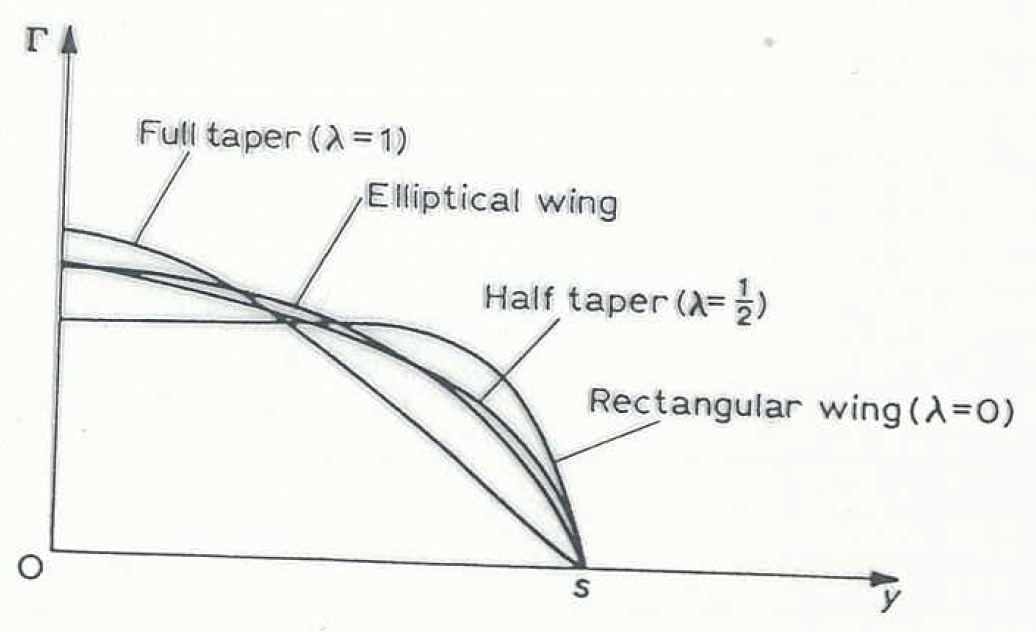
\includegraphics[scale=0.15]{ch3/23}
		\captionof{figure}{}	
		\label{fig:3.23}
	\end{minipage}
	\begin{minipage}{0.22\textwidth}
		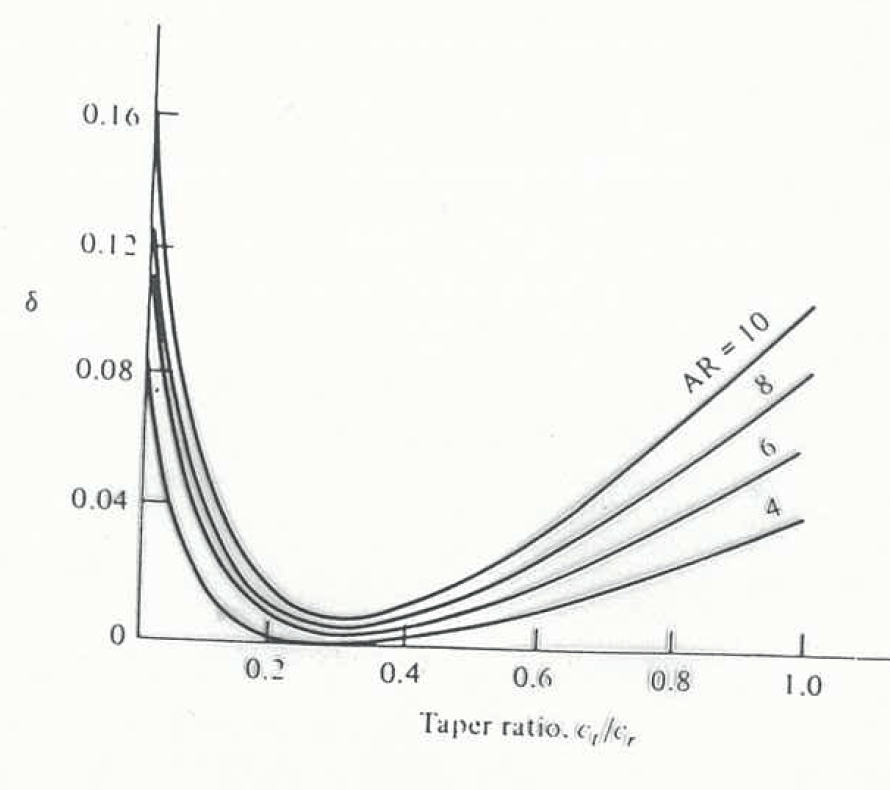
\includegraphics[scale=0.12]{ch3/24}
		\captionof{figure}{}	
		\label{fig:3.24}
	\end{minipage}
\end{center}

After some calculation one find a circulation distribution as in \autoref{fig:3.23}, where $\lambda$ is defined such that $c_t = (1- \lambda) c_r$. $\lambda = 0$ corresponds to a rectangular wing and $\lambda = 1$ is the triangular one. Note that the figure also represents the lift. The lift coefficient no, because it becomes larger at the tips due to $c\searrow$. On \autoref{fig:3.24} is represented the induced drag coefficient $\delta$. We see that it is always possible to find the taper ratio to have the minimum drag. Most of the planes use tapered wings since it is more simple to produce than elliptic wing.

\subsection{Assume an elliptic distribution for the circulation. Show that the platform of the
	wing must be an ellipse.}

The elliptic circulation distribution is written:

\begin{equation}
\Gamma (y) = \Gamma (y_0) \sqrt{1-\left( \frac{y}{b/2} \right)^2}.
\end{equation}

where $\Gamma _0$ is the circulation in the plane of symmetry. Let's compute the velocity:

\begin{equation}
v(y_0) = \frac{1}{4\pi} \int _{-b/2}^{b/2} \frac{d\Gamma }{y_0 - y} = \frac{\Gamma _0}{2b} = cst \qquad \Rightarrow \epsilon = \alpha _i = \frac{v(y_0)}{v_\infty} = \frac{\Gamma _0}{2b v_\infty} = cst.
\end{equation}

where we used the transformation $y = b/2 \cos \theta$. Induced angle of attack is constant along the span.

\begin{equation}
L'(y) = \rho v_\infty \sqrt{1-\left( \frac{y}{b/2} \right)^2}.
\end{equation}

On the other hand we can use \eqref{eq:3.4} to express the lift as: 

\begin{equation}
L'(y) = m (\alpha - \alpha _i - \alpha _0) \frac{1}{2} \rho _\infty v_\infty ^2 c
\end{equation}

Combining the equations we get: 

\begin{equation}
(\alpha - \alpha _i - \alpha _0) c = \frac{2\Gamma _0}{v_\infty} \sqrt{1-\left( \frac{y}{b/2}\right)^2}. 
\end{equation}

Note that if the left hand side is constant, the equation is satisfied for an \textbf{elliptic platform}. Since $\alpha _i$ is already constant, the whole term is constant only if the geometric angle of attack is constant and the profile does not change along the span. Since $C_{d_i} = C_L \alpha _i$, we can make the same analysis for the drag. \\

On the other hand, if the platform is non elliptic, since m varies little, the different angles must vary too. This is done by introducing a \textbf{twist} in the wing so that $\alpha$ varies. The lift coefficient is obtained by integration of the local lift:

\begin{equation}
\frac{1}{\frac{1}{2}\rho v_\infty ^2 S} \int _{-b/2}^{b/2} L'(y) \, dy = \frac{\Gamma _0\pi b}{2v_\infty S} = \frac{\Gamma _0 \pi}{2bv_\infty} AR.
\end{equation}

Combination of this and what we found for $\alpha _i$ in this section we get:

\begin{equation}
\alpha _i = \frac{C_L}{\pi AR}
\end{equation}

which is what we defined at the beginning of the chapter but for $e =1$ (span efficiency factor). The induced drag is given by:

\begin{equation}
D_i'(y) = L'(y) \alpha _i \qquad \Rightarrow C_{D_i} = C_L \alpha _i = \frac{C_L^2}{\pi AR}.
\end{equation}


%-----------------------------------------------------------------------------------------------------------------
%-----------------------------------------------------------------------------------------------------------------
%-----------------------------------------------------------------------------------------------------------------

\section{2D airfoil in compressible flow}
\subsection{Derive the compressible potential equation}
TODO

\subsection{Assume a thin airfoil at small angle of attack: derive the linearized potential
	equation. What is the range of validity as a function of the free stream Mach
	number}
TODO

\subsection{Discuss the type of this equation as a function of free stream Mach number,
	what are the consequences}
TODO

%-----------------------------------------------------------------------------------------------------------------
%-----------------------------------------------------------------------------------------------------------------
%-----------------------------------------------------------------------------------------------------------------

\section{2D airfoil compressible flow around an airfoil using the small perturbation
	approach}

\subsection{Derive the equation governing compressible potential equation, what are the
	assumptions}

Remind that we have defined a potential function to describe incompressible flows, conservation of mass giving:

\begin{equation}
\vec{v} = \nabla \phi \qquad \frac{\D u}{\D x} + \frac{\D v}{\D y} = 0 = \frac{\D^2 \phi}{\D x^2} + \frac{\D^2 \phi}{\D y^2}.
\end{equation}

This can also be used to describe compressible flows, conservation of mass is then: 

\begin{equation}
\rho (\phi _{xx} + \phi _{yy}) + \rho _x \phi _x + \rho _y \phi _y = 0
\label{eq:6.2}
\end{equation}

where we introduced the shorthand notation $\frac{\D a}{\D x} = a_x$. We assume that the flow is isentropic, this is satisfied by inviscid flows (no shock  wave): 

\begin{equation}
\frac{\rho}{T^{\frac{1}{\gamma -1}}} = cst \qquad \Rightarrow \frac{d \rho}{\rho} = \frac{1}{\gamma -1} \frac{dT}{T}
\end{equation}

if the flow does not work (turbine), the temperature is constant and the equation becomes:

\begin{equation}
d\rho = -\frac{\rho}{2a^2} d(u^2+v^2).
\end{equation}

If we replace the velocities we get: 

\begin{equation}
\rho _x = -\frac{\rho}{a^2} (\phi _x \phi _{xx} + \phi _y \phi _{xy}) \qquad \rho _y = -\frac{\rho}{a^2} (\phi _x \phi _{xy} + \phi _y \phi _{yy}).
\end{equation}		

That we can substitute in \eqref{eq:6.2}:

\begin{equation}
\left( 1-\frac{1}{a^2} \phi^2_x \right) \phi _{xx} + \left( 1-\frac{1}{a^2 }\phi^2_y \right) \phi _{yy} - \frac{2}{a^2} \phi_x \phi_y \phi _{xy} = 0.
\label{eq:6.6}
\end{equation}	


\subsection{Derive the equation in the case of small perturbations. What are the assumptions
	for this equation to be valid ?}

If the far field velocity profile is $u= V_\infty$, we can note the velocity field by means of perturbations: $u = V_\infty + \hat{u}, v = \hat{v}$. A perturbation potential function can be defined: 

\begin{equation}
\phi = V_\infty x + \hat{\phi}\qquad with \qquad \hat{\phi} _x = \hat{u}, \quad \hat{\phi}_y = \hat{v}. 
\end{equation}

By substitution of this in \eqref{eq:6.6}:

\begin{equation}
\left[ a^2- (V_\infty + \hat{\phi} _x )^2 \right] \hat{\phi} _{xx} + \left[ a^2-\hat{\phi}_y ^2 \right] \hat{\phi} _{yy} - 2 (V_\infty + \hat{\phi} _x) \hat{\phi}_y \hat{\phi} _{xy} = 0.
\label{eq:6.8}
\end{equation}

Since the total temperature is constant:

\begin{equation}
\frac{a^2_\infty}{\gamma -1} + \frac{V_\infty ^2}{2} = \frac{a^2}{\gamma -1} + \frac{(V_\infty + \hat{u}) ^2 = \hat{v}^2}{2} 
\label{eq:6.9}
\end{equation}

If we make the assumption of small perturbation, the quadratic terms cancel and \eqref{eq:6.8} and \eqref{eq:6.9} become:

\begin{equation}
\begin{aligned}
&\frac{a^2_\infty}{a^2} = 1 - (\gamma -1) \frac{\hat{u}}{V_\infty} M^2_\infty\\
&\left[ a^2- V^2_\infty + 2V_\infty \hat{u}  \right] \hat{\phi} _{xx} + a^2 \hat{\phi} _{yy} - 2 V_\infty \hat{v} \hat{\phi} _{xy} = 0 \\ 
\Rightarrow 
&\left[ 1- M_\infty^2 - (\gamma + 1) M_\infty \frac{\hat{u}}{V_\infty} \right] \hat{\phi} _{xx} + \left[ 1 - (\gamma -1 )M_\infty ^2\frac{\hat{u}}{V_\infty} \right] \hat{\phi} _{yy} - 2 M^2_\infty \frac{\hat{v}}{V_\infty} \hat{\phi} _{xy} = 0 
\end{aligned}
\end{equation}

where the last expression is obtained by dividing by $a^2_\infty$ and replacing. By considering again the small perturbation ($V_\infty \ll$) equation we get the:

\begin{center}
	\theor{
		\textbf{Transonic smal perturbation potential equation}
		\begin{equation}
		\left[ (1-M_\infty ^2) - (\gamma +1) M^2_\infty \frac{\hat{\phi}_x}{V_\infty}  \right] \hat{\phi} _{xx} + \hat{\phi} _{yy} = 0.
		\end{equation}
	}
\end{center}

We can see that the $\hat{u}$ appears in $\hat{phi} _{xx}$ term, this is no longer negligible for \textbf{sonic} velocities. For sub- and super-sonic flows however the equation simplifies in: 

\begin{equation}
(1-M_\infty ^2) \hat{\phi} _{xx} + \hat{\phi} _{yy} = 0.
\end{equation}

Note that we retrieve our incompressible equation for $M_\infty \rightarrow 0$. Be aware that this last relation is only valid for small perturbations (small bodies in practice) and sub- or super-sonic flows ($M_\infty > 1.2, M_\infty < 0.8$). \\

Let's now operate a change of coordinate $(x,y) \rightarrow (\xi , \eta)$, recalling $1-M_\infty ^2 \equiv \beta ^2$: 

\begin{equation}
\xi = x \quad \eta = \beta y \qquad \bar{\phi} (\xi , \eta) = m .\hat{\phi}(x,y)
\end{equation}

where m is a constant. Let's find the expression of $\bar{\phi} (\xi, \eta)$. The chain rule gives: 

\begin{equation}
\begin{aligned}
\hat{\phi} _x = \hat{\phi}_\xi = \frac{1}{m} \bar{\phi} _\xi \qquad  \hat{\phi} _y = \frac{\beta}{m} \bar{\phi}_\eta &\qquad \hat{\phi} _{xx} = \frac{1}{m} \bar{\phi}_{\xi \xi} \qquad \hat{\phi} _{yy} = \frac{\beta ^2}{m} \bar{\phi}_{\eta \eta}\\
&\Rightarrow \bar{\phi}_{xx} + \bar{\phi}_{yy} = 0
\end{aligned}
\label{eq:6.14}
\end{equation}

We can see that the compressible flow in $(x,y)$ is reduced to an incompressible flow in the $(\xi, \eta)$ plane. Pay attention that $\bar{\phi}$ describes the perturbation velocities $\bar{u}, \bar{v}$. in the $(\xi, \eta)$ plane.  

\wrapfig{7}{l}{7.5}{0.1}{ch6/9}{fig:6.9}
We can now focus on the shape of the profile in the new axis. Let's analyze the tangent to the profile by defining the angle $\theta$ for the profile in (x,y). Under the assumption of small perturbation (thin airfoil), we can see that:

\begin{equation}
\tan \theta \approx \theta = \frac{\hat{v}}{V_\infty + \hat{u}} \approx \frac{\hat{v}}{V_\infty} = \frac{1}{V_\infty} \hat{\phi} _y \qquad \Rightarrow \chi \approx \frac{1}{V_\infty} \bar{\phi} _\eta
\end{equation}

where the analogy for the new plane is done. Using \eqref{eq:6.14}, we get: 

\begin{equation}
\theta = \frac{\beta}{m} \chi.
\end{equation}

Let's investigate two cases: 
\begin{itemize}
	\item[•] If we choose $m=\beta$, $\theta = \chi$, the two profiles are identical. We have for the velocity: 
	
	\begin{equation}
	\hat{u} = \hat{\phi} _x = \frac{\bar{\phi}_\xi}{\beta} = \frac{\bar{u}}{\beta}
	\end{equation}
	
	and since the pressure coefficient is given by $C_p = -\frac{2\hat{u}}{V_\infty}$: 
\end{itemize}		

\begin{center}
	\theor{
		\textbf{Prandtl-Glauert rule}
		\begin{equation}
		C_p = \frac{C_{p,inc}}{\beta} = \frac{C_{p,inc}}{\sqrt{1 - M_\infty ^2}}.
		\end{equation}
		This equation allows us to compute the pressure distribution in compressible flow, beginning from the incompressible one. 
	}
\end{center}


\wrapfig{12}{r}{5}{0.15}{ch6/10}{fig:6.10}
Since the lift and moment coefficient are given by the integration of the pressure coefficient along the wing, we have the same result for them (so also the slope of lift curve $m$). Here is plotted the experimental data and the approximated m by means of the above relation for $\alpha = 0$ and for different airfoil thickness $\tau$. We can see that for the thinner wings, we have a good agreement, until we reach the \textbf{critical Mach number} (Mach number at infinity for which Mach number 1 is reached on the profile).  This value exceeded, we have shock waves (formula valid only for Mach until 0.8). 
For thicker wings, we see that the slope m is always underestimated. The critical Mach number is here much lower. 

\ \\
\begin{itemize}
	\item[•] If we choose $m=1, \hat{u} = \bar{u}$ so that $C_p = C_{p, inc}$. We see that the pressure coefficient is now the same but the profiles are different following we are in the compressible or incompressible case $\theta = \beta \chi$. 
\end{itemize}

\wrapfig{5}{l}{6.5}{0.1}{ch6/11}{fig:6.11}
The angle relation must be true along the entire profile, particularly at the maximum thickness: 

\begin{equation}
\tau = \beta \tau _{inc}. 
\end{equation}		

\paragraph{Remark 1}
If we take into account the aspect ratio, we can rewrite the slope m as: 

\begin{equation}
m = \frac{m_{inc}}{\beta} \frac{2\pi}{\beta \left(1+\frac{2}{eAR}\right)}
\end{equation}		

where we used the theoretical 2D slope $2\pi$. Another possibility is to write the lift as:

\begin{equation}
c_l = \frac{2\pi}{\beta} (\alpha - \alpha _{L_0} - \alpha _i) = \frac{2\pi}{\beta+\frac{2}{eAR}} (\alpha - \alpha _{L_0})
\end{equation}

We can	last note the existence of the DATCOM formula that accounts for the effect of the aspect ratio, sweep angle $\Lambda$, Mach number and has also a correction factor for viscous effects $\kappa \approx 0.97$: 

\begin{equation}
m = \frac{2\pi AR}{2+\sqrt{\frac{AR^2 + beta ^2}{\kappa ^2}\left( 1+\frac{\tan ^2\Lambda}{\beta ^2} \right)+4}}.
\end{equation}

\paragraph{Remark 2}
We can also rearrange the expression of $C_p$ with the approximation of small angles, we had: 

\begin{equation}
C_p = \frac{p-p_\infty}{\frac{1}{2}\rho _\infty V_\infty^2} = \frac{\gamma 2p_\infty}{\gamma \rho _\infty V_\infty ^2}\left(\frac{p}{p_\infty}-1 \right) =  \frac{2}{\gamma M^2_\infty} \left(\frac{p}{p_\infty} -1 \right) \qquad \gamma \frac{p_\infty}{\rho _\infty} = \gamma rT = a^2
\label{eq:6.23}
\end{equation}

The isentropic flow and the constant $T_c$ give: 

\begin{equation}
\begin{aligned}
&\frac{p}{p_\infty}  =\left( \frac{T}{T_\infty} \right) ^{\frac{\gamma}{\gamma - 1}} = \left( \frac{T_t - \frac{1}{2c_p}\left[ (V_\infty +\hat{u})^2 +\hat{v}^2 \right]}{T_\infty} \right)^{\frac{\gamma}{\gamma-1}} \qquad T_t = T_\infty + \frac{V_\infty^2}{2c_p}\\
\Rightarrow &\frac{p}{p_\infty}  =\left[ 1- \frac{\gamma -1}{2}M^2_\infty \left( \frac{2\hat{u}}{V_\infty} +\frac{\hat{u}^2 +\hat{v}^2}{V^2_\infty} \right) \right]^{\frac{\gamma}{\gamma-1}} = 1- \frac{\gamma}{2}M^2_\infty \left( \frac{2\hat{u}}{V_\infty} +\frac{\hat{u}^2 +\hat{v}^2}{V^2_\infty} \right)+\dots
\end{aligned}
\end{equation}

where the last expression comes from the fact that the second term is small so that we have the Taylor development of $1+\epsilon$ (first order limited). We can neglect the second term in bracket since we have small perturbation square, and we get by \eqref{eq:6.23}:

\begin{equation}
\frac{p}{p_\infty} = -\frac{2\hat{u}}{V_\infty}
\end{equation}

\subsection{Discuss the application to an airfoil in supersonic flow: lift coefficient, influence
	of the Mach number, Ackeret formula, lift and drag formula}

The potential equation we used in the framework of potential equation can be rewritten in the case of supersonic flow as:

\begin{equation}
(1-M_\infty^2) \hat{\phi}_{xx} + \hat{\phi}_{yy} = 0 \qquad \Rightarrow \lambda ^2 \hat{\phi} _{xx} - \hat{\phi} _{yy} = 0.
\end{equation}

The linearized potential equation corresponds to the wave equation with $\lambda ^2 = M_\infty ^2 -1 >0$. We can show that the solution of this equation is 

\begin{equation}
\hat{\phi}(x,y)= f(x-\lambda y) = \hat{\phi} _{1}(x-\lambda y) + \hat{\phi} _{2} (x+\lambda y).
\end{equation}		

Let's define 2 families of characteristic curves:

\begin{equation}
\left\{
\begin{aligned}
&C^+ : x-\lambda y = cst \qquad \Rightarrow y = \frac{1}{\lambda} x + cst = \frac{1}{\sqrt{M_\infty ^2 -1}} c + cst\\
&C^+ : x+\lambda y = cst \qquad \Rightarrow y = -\frac{1}{\lambda} x + cst = -\frac{1}{\sqrt{M_\infty ^2 -1}} c + cst
\end{aligned}
\right.
\end{equation}

\wrapfig{8}{r}{5}{0.15}{ch6/8}{fig:6.8}
In this way, $\hat{\phi} _1$ and $\hat{\phi} _2$ are respectively constant on $C^+$ and $C^-$. The slope is denoted $\mu _\infty ^\pm$ for $C^\pm$ such that: 

\begin{equation}
\tan \mu _\infty ^\pm = \pm \frac{1}{\sqrt{M_\infty ^2 -1}} \qquad \sin \mu _\infty ^\pm = \pm \frac{1}{M_\infty}.
\end{equation}

To find the general solution in P, let's first consider the initial data given on the y-axis: 

\begin{equation}
\hat{\phi} _1(y) = F(y)\qquad \hat{\phi}_2 (y) = G(y)
\end{equation}

Now let's construct $C^+$ and $C^-$ : 

\begin{equation}
C^+ : x-\lambda y = x_A - \lambda y_A\qquad C^- : x-\lambda y = x_B + \lambda y_B.
\end{equation}

Finally, the solution in P is so given by:

\begin{equation}
\hat{ \phi} (x_p,y_p) = \hat{\phi} (x_A - \lambda y_A) + \hat{\phi} _2 (x_B + \lambda y_B) = F (x_A - \lambda y_A) + G (x_B + \lambda y_B)
\end{equation}

\wrapfig{8}{l}{5}{0.1}{ch6/17}{fig:6.17}
Now let's define the initial conditions at $x=0$ for small $\alpha$ for a thin profile:

\begin{equation}
F(y) = K_1 = cst \qquad G(y) = K_2 = cst \qquad \Rightarrow \hat{\phi} = cst
\end{equation}

since the incoming flow is uniform. On the pressure side, we have $\hat{\phi} _1(x-\lambda y) = K_1$ which gives in the solution: 

\begin{equation}
\hat{\phi}(q) = K_1 + \hat{\phi}_2 (q) \qquad \rightarrow \hat{\phi}_x = \frac{d\hat{\phi}_2}{dq} = \hat{u} ^- \quad \hat{\phi}_y = \frac{d\hat{\phi}_2}{dq}\lambda = \hat{v} ^- \qquad \Rightarrow \hat{v}_{wall} = \lambda \hat{u}_{wall}
\end{equation}

If we express the tangent as $\tan \theta_w \approx \theta_w = \frac{\hat{v}^-_w}{\hat{u}^-+V_\infty} \approx \frac{\hat{v}^-_w}{V_\infty}$,
We can get by replacing the last results in the previous pressure coefficient equation for small perturbations:


\begin{center}
	\theor{
		\textbf{Law of Ackeret}
		\begin{equation}
		C_p ^- = -\frac{2\hat{u}^-_w}{V_\infty} = -\frac{2\theta_w^-}{\sqrt{M^2_\infty - 1}}.
		\end{equation}
	}
\end{center}

The same reasoning can be done for the suction side where we'll get:

\begin{equation}
\hat{\phi} _x = \frac{d\hat{\phi}_1}{dq} = \hat{u}^+_w \qquad \hat{\phi} _x = \frac{d\hat{\phi}_1}{dq}(-\lambda) = \hat{v}^+_w = -\lambda \hat{u}^+_w\qquad \Rightarrow C_p^+ = \frac{2\theta_w^+}{\sqrt{M^2_\infty - 1}}.
\end{equation}

\subsubsection{Application to a flat plate}
\wrapfig{8}{l}{7.5}{0.1}{ch6/18}{fig:6.18}
Consider the thin profile define by functions $y^+(x)$ and $y^-(x)$ with angles defines as:

\begin{equation}
\begin{aligned}
&\epsilon = \frac{dy}{dx} <0 \qquad \theta = \frac{\hat{v}}{\hat{u} +V_\infty} <0 \\
\Rightarrow &\theta = \epsilon - \alpha = \frac{dy}{dx} - \alpha
\end{aligned}
\end{equation}

as $\alpha > 0$. We can then apply the last formula: 

\begin{equation}
C_p^+ = \frac{2\theta_w^+}{\sqrt{M^2_\infty - 1}} = \frac{2\left( \frac{dy^+}{dx} -\alpha \right)}{\sqrt{M^2_\infty - 1}} \qquad C_p^- = -\frac{2\theta_w^-}{\sqrt{M^2_\infty - 1}} = \frac{2\left( \alpha -\frac{dy^-}{dx}\right)}{\sqrt{M^2_\infty - 1}}.
\end{equation}

We are now interested in computing the normal and tangential force applied on the wing, for a counter-clock contour: 

\begin{equation}
C_N = \int _0 ^1 C_p ^- \, \frac{dx}{c} + \int _1 ^0 C_p ^+ \, \frac{dx}{c} = \frac{4\alpha }{\sqrt{M_\infty ^2-1}}
\end{equation}

where we replace the $C_p$'s by their definition and we neglect $\frac{dy}{dx}$ terms. For the drag we have the same procedure but by neglecting this time $\alpha$:

\begin{equation}
\begin{aligned}
&C_\Gamma = -\int _0 ^1 C_p ^- \, \frac{dy}{c} - \int _1 ^0 C_p ^+ \, \frac{dy}{c} = \frac{2}{\sqrt{M_\infty ^2-1}} \left[ \int _0^1 \left(\frac{dy^-}{dx} \right)^2 \frac{dx}{c} + \int _0^1 \left(\frac{dy^+}{dx} \right)^2 \frac{dx}{c} \right]\\
\Rightarrow &C_\Gamma =  \frac{2}{\sqrt{M_\infty ^2-1}} [I^- + I^+]
\end{aligned}
\end{equation}

To compute the lift and drag coefficient we only have to make the projections, and in case of flat plate $\frac{dy}{dx} = 0 = I^\pm$: 

\begin{equation}
\begin{aligned}
&C_l = -C_\Gamma \sin \alpha + C_N \cos \alpha \approx -\alpha C_\Gamma  + C_N \qquad C_d = C_\Gamma  + \alpha C_N\\
\Rightarrow &C_l = \frac{4\alpha}{\sqrt{M_\infty ^2 -1}} \qquad C_d = \frac{4\alpha}{\sqrt{M_\infty ^2 -1}}.
\end{aligned}
\end{equation}

The drag is the \textbf{wave drag}.

\subsection{What is wave drag ? discuss supersonic flow over double wedge profile}
A wave drag is a drag due to a shock wave. When a shock wave appears, it uses energy, which has to be provided by the aircraft, it is thus seen as a drag.

\wrapfig{8}{r}{6.5}{0.1}{ch6/19}{fig:6.19}
If we apply the Ackeret law to this profile we have:

\begin{equation}
\begin{aligned}
&C_{p1} = \frac{2(\delta - \alpha)}{\sqrt{M_\infty^2 -1}} \qquad C_{p2} = \frac{2(\delta + \alpha)}{\sqrt{M_\infty^2 -1}} \\
&C_{p3} = \frac{-2(\delta + \alpha)}{\sqrt{M_\infty^2 -1}} \qquad C_{p4} = \frac{-2(\delta - \alpha)}{\sqrt{M_\infty^2 -1}}
\end{aligned}
\end{equation}

We can compute the lift and drag coefficients by integrating over the surface:

\begin{equation}
\begin{aligned}
&\vec{F} = -\oint p\, d\vec{S} = -\oint (p-p_\infty)\, d\vec{S} = -\frac{1}{2} \rho _\infty V_\infty ^2 \oint C_p\, d\vec{S}\\
\Rightarrow &\vec{F}_1 = -\frac{1}{2} \rho _\infty V_\infty ^2 C_{p1} \frac{c}{2} \vec{n}_1
\end{aligned}
\end{equation}

If we make the force non dimensional: 
\begin{equation}
\vec{C}_1 = \frac{\vec{F}_1}{\frac{1}{2}\rho _\infty V_\infty ^2 c} = -\frac{C_{p1}}{2} \vec{n}_1 \qquad \Rightarrow \vec{C}_i = -\frac{C_{pi}}{2} \vec{n}_i
\end{equation}

If we look to the normal and tangent forces we find: 

\begin{equation}
\begin{aligned}
C_y = \vec{C}_i .\vec{1}_y = \left(-\frac{C_{p1}}{2} + \frac{C_{p2}}{2} -\frac{C_{p3}}{2} +\frac{C_{p4}}{2} \right) \cos \delta= \frac{4\alpha }{\sqrt{M_\infty ^2 -1}} \cos \delta \approx \frac{4\alpha }{\sqrt{M_\infty ^2 -1}}\\
C_x = \vec{C}_i .\vec{1}_x = \left(\frac{C_{p1}}{2} + \frac{C_{p2}}{2} -\frac{C_{p3}}{2} -\frac{C_{p4}}{2} \right) \sin \delta = \frac{4\delta }{\sqrt{M_\infty ^2 -1}} \sin \delta \approx \frac{4\delta ^2}{\sqrt{M_\infty ^2 -1}}
\end{aligned}
\end{equation}

Then we make the same projection as previously: 

\begin{equation}
c_l \approx C_y - \alpha C_x = \frac{4\alpha }{\sqrt{M_\infty ^2 -1}} - \frac{4\delta ^2\alpha }{\sqrt{M_\infty ^2 -1}}  \approx \frac{4\alpha }{\sqrt{M_\infty ^2 -1}} 
\end{equation}

We find thus the same lift coefficient as the flat plate. Let's see the drag: 

\begin{equation}
c_d = C_x + \alpha C_y = \frac{4\alpha }{\sqrt{M_\infty ^2 -1}} + \frac{4\delta}{\sqrt{M_\infty ^2 -1}},
\end{equation}

\wrapfig{11}{l}{3}{0.3}{ch6/20}{fig:6.20}
where the first term is \textbf{incidence wave drag} (result of lift), the same as the flat plate and the second term the \textbf{thickness wave drag} (result of volume) corresponding to the drag of the wedge at 0 degrees and angle of attack. The following empirical formula can be used for both drag on wing and on \textbf{complete plane}: 

\begin{equation}
C_{Dw} = k_0 \frac{128}{\pi} \frac{V^2}{Sl^4} + k_1 \frac{1}{2\pi} \frac{S}{l^2}\lambda ^2 C_L^2
\end{equation}

where $k_0$ and $k_1$ are constant of order 1 depending on the geometry and l the average length as represented on the figure. 

\subsection{Transonic flow over a profile: what is critical free stream Mach number(+ discussion), what is
	drag divergence Mach number}
\subsubsection{Critical Mach number}
The critical Mach Number is the $M_\infty$ when $M = 1$ somewhere on the airfoil. Consider a point A, the drag is given by: 

\begin{equation}
C_{p,A} = \frac{2}{\gamma M_\infty^2} \left( \frac{p_A}{p_\infty} -1 \right)
\end{equation}

If we combine the fact that the flow is isentropic:

\begin{equation}
\frac{p_A}{p_\infty} = \left(\frac{T_A}{T_\infty}\right)^{\frac{\gamma}{\gamma -1}} = \left(\frac{1+\frac{\gamma - 1}{2}M^2_\infty}{1+\frac{\gamma - 1}{2}M^2_A}\right)^{\frac{\gamma}{\gamma -1}} 
\quad \Rightarrow C_{p,A} = \frac{2}{\gamma M_\infty^2} \left[ \left(\frac{1+\frac{\gamma - 1}{2}M^2_\infty}{1+\frac{\gamma - 1}{2}M^2_A}\right)^{\frac{\gamma}{\gamma -1}} -1 \right]
\end{equation}

If now we consider $M_\infty = M_{kr} \rightarrow M_A = 1$, so that the equation becomes: 

\begin{equation}
C_{p,A} = \frac{2}{\gamma M_\infty^2} \left[ \left(\frac{1+\frac{\gamma - 1}{2}M^2_\infty}{1+\frac{\gamma - 1}{2}M^2_A}\right)^{\frac{\gamma}{\gamma -1}} -1 \right] \qquad C_{p,A} = \frac{C_{p,A,inc}}{\sqrt{1-M_{kr}^2}},
\end{equation}


\wrapfig{10}{r}{5}{0.15}{ch6/13}{fig:6.13}
where the second equation is the Prandtl-Glauert relation. 
We can plot the two equations on a graph. The intersection of the two graphs gives the critical Mach number. We can see that the minimum lift coefficient at low velocities is more negative than the thin case, characterized by a smaller $M_{kr}$. The perturbation of the flow is higher. Flying at high subsonic velocities is important $\rightarrow$ thin airfoil. When the angle of attack increases, the lift increases but the higher velocity on the suction part makes the $M_{kr}$ much lower. We want so the wing to be as thin as possible but we are limited by the structural strength and the fuel storage.

\ \\
\wrapfig{10}{l}{4.5}{0.1}{ch6/14}{fig:6.14}
We avoid also large bending of the leading edge to avoid large accelerations. One solution to increase $M_{kr}$ is to place the maximum camber downstream, about 50\% of the chord because the velocities on the suction side will be lower. Placing it too downstream will create a too high opposite gradient and cause separation. 

\ \\ Symmetrical wings have a larger $M_{kr}$, however be careful with combination of sharp LE because of LE separation. In practice we have a quasi-symmetrical profile with camber near LE. \textbf{Swept} wings also increase the $M_{kr}$. 

\minifig{ch6/15}{ch6/16}{0.2}{0.15}{0.45}{0.3}

We wan observe here above, the plot of $\alpha, C_L$ and $C_D$ for a symmetrical and a non-symmetrical airfoil. We can observe on \autoref{ch6/15} that the slope of the lift curve goes up to $M=0.83$ (Prandtl-Glauert). Once above $M_{kr}$ it starts to decrease and the drag suddenly increases. \\

On \autoref{ch6/16} we can see similar effects at the difference that around $M_{kr}$ we have a positive increase of the zero lift angle, having a negative effect on longitudinal stability. Note that the decrease of the lift curve starts earlier, $M_{kr}$ is smaller. 

\subsubsection{Drag divergence Mach number}
\wrapfig{22}{l}{4.5}{0.2}{ch6/1}{fig:6.1}
At the critical Mach number $M_\infty = M_{cr}$, the flow reaches $M=1$ somewhere on the wing. If the velocity at $\infty$ is increased, $M_\infty$ also (still <0), a small area where the flow becomes \textbf{supersonic} will develop on the \textbf{suction side}. For increasing $M_\infty$ this area will growth and at a certain $M_\infty$ a \textbf{shock wave} will develop, as a result of which the flow will become \textbf{subsonic} again (the supersonic area abruptly terminated). Such area also develops on the \textbf{pressure side} at high $M_\infty$ (\autoref{fig:6.1} (a)).

\ \\ If $M_\infty$ increases further, the supersonic regions further extends and the shock waves moves downstream, the one on the pressure side more rapidly (\autoref{fig:6.1} (b) (c)). As soon as the shock waves are strong enough, they can cause separation of the boundary layer, this separation is the \textbf{shock stall} and the $M_\infty$ where this happen is called the \textbf{drag divergence Mach number}. Indeed, the drag suddenly increases as result of the separation, this called \textbf{transonic drag rise}, shown on \autoref{fig:6.2}. 

\ \\ For further increase of $M_\infty <1$, the shock wave on the pressure side eventually reaches the trailing edge (\autoref{fig:6.1} (d)). In a certain Mach number range, the shock wave manifests the so-called $\bm{\lambda}$ \textbf{shocks}. Near the profile the shock has two legs, a first oblique one through which the flow is slowed down but remains supersonic, and a second normal one through which the flow becomes subsonic. 

\ \\ Eventually the shock wave on the suction side can also reach the trailing edge and give birth to the \textbf{bifurcated trailing edge shock} patern (\autoref{fig:6.1} (e)). 

\ \\ For further increase of $M_\infty$ there is no change, till $M_\infty$ exceeds 1. In this case, a so-called \textbf{detached bow shock} develops upstream of the leading edge. There is a small subsonic region between this shock and the leading edge. This manifests both for thick, bounded leading edge and thin one (\autoref{fig:6.1} (f) (g)). In the second case, the bow shock changes into 2 oblique shocks at the leading edge for increasing $M_\infty$ (\autoref{fig:6.1} (h)). This happens at the \textbf{shock attachment Mach number}, $\bm{M_{SA}}$. For further $M_{\infty}$, the flow becomes fully supersonic and the drag decreases. In the case of rounded leading edge, the bow shock continues to exist and comes closer to the leading edge. 

\begin{center}
	\begin{minipage}{0.3\textwidth}
		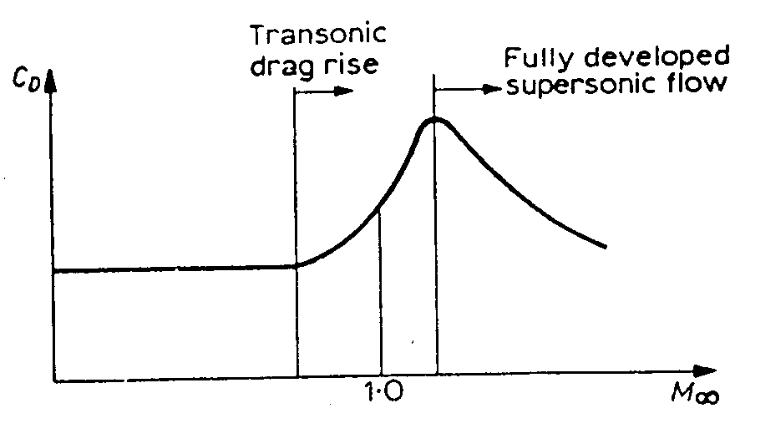
\includegraphics[scale=0.15]{ch6/2}
		\captionof{figure}{}
		\label{fig:6.2}
	\end{minipage}
	\begin{minipage}{0.3\textwidth}
		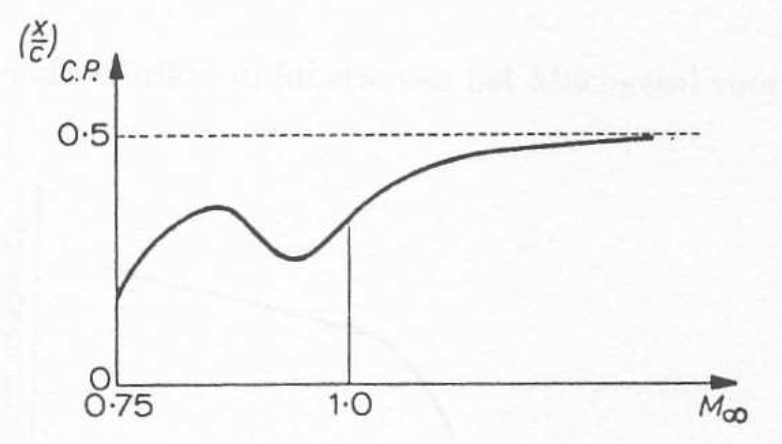
\includegraphics[scale=0.15]{ch6/3}
		\captionof{figure}{}
		\label{fig:6.3}
	\end{minipage}
\end{center}

Under transonic conditions the flow is non-stationary, the shock waves moves up and down on the wing. The pilot senses this as \textbf{buffeting} (response of the structure to aerodynamic excitation) and vibrations. This can make the plane uncontrollable or cause serious damages. The cause of the excitation is the fluctuating pressure in non-stationary conditions. Normally one flies under the buffeting margin but one can exceed it in case of sudden maneuvers for fighters for example. \\

The center of pressure is also moving with $M_\infty$ (\autoref{fig:6.3}). First, it goes backward as the shock wave going backward on the suction side makes the underpressure greater. Then, it goes forward because the shock wave on the pressure side is moving faster. The latter reaches the trailing edge while the shock wave on the suction side still moves backward, making the center of pressure again move backward, tending to the 50\% chord. This makes the control of the plane more difficult. \\

\wrapfig{7}{l}{5.5}{0.15}{ch6/4}{fig:6.4}
It is this buffeting effect that imposes an upper limit to the velocity of subsonic planes. With the increase of the drag due to separation when shock waves (shock-stall) is associated a decrease of the lift. We can see that the lift temporary increases after the lower shock reaches the trailing edge. This is explained by the smaller separation when in this location. The drag divergence Mach number is 5-10\% larger than $M_{cr}$. 

\ \\

\begin{center}
	\begin{minipage}{0.4\textwidth}
		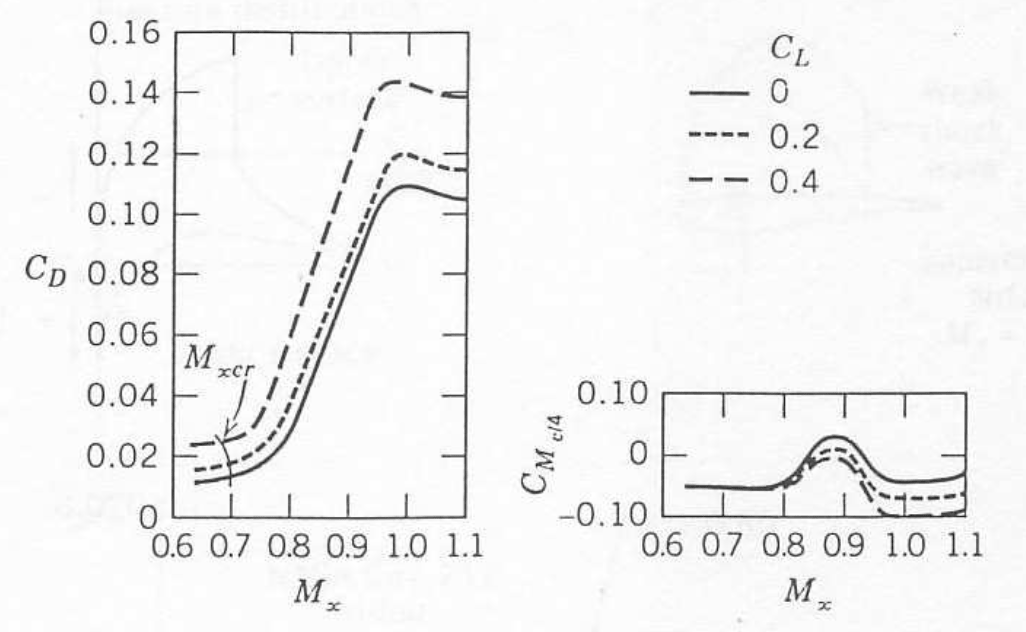
\includegraphics[scale=0.15]{ch6/5}
		\captionof{figure}{}
		\label{fig:6.5}
	\end{minipage}
	\begin{minipage}{0.4\textwidth}
		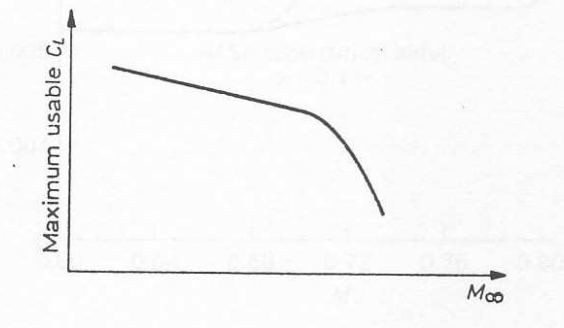
\includegraphics[scale=0.4]{ch6/6}
		\captionof{figure}{}
		\label{fig:6.6}
	\end{minipage}
\end{center}

On \autoref{fig:6.5} we can see the influence of increasing lift (increasing $\alpha$). We can notice that with increasing lift, the drag increases for all Mach numbers, the moment increases in the transonic region and $M_{cr}$ decreases. On \autoref{fig:6.6}, we notice that the lift coefficient strongly decreases in the transonic region due to buffering effects. 


\subsection{Compute the lift coefficient for a 2D profile in compressible flow, assuming
	that the lift coefficient for the same airfoil is known for incompressible flow.}
Using Prandtl-Glauert : $C_p = \frac{C_{p,inc}}{\beta} = \frac{C_{p,inc}}{\sqrt{1 - M_\infty ^2}}$. Since lift is an integration of pressure: $C_L = \frac{C_{L,inc}}{\beta} = \frac{C_{L,inc}}{\sqrt{1 - M_\infty ^2}}$


\subsection{Discuss the graph giving the slope of the lift curve as a function of the free
	stream Mach number ($M_{infinity}$)}

TODO
%-----------------------------------------------------------------------------------------------------------------
%-----------------------------------------------------------------------------------------------------------------
%-----------------------------------------------------------------------------------------------------------------

\section{Discuss effect of sweep on performance of a 3D wing in compressible flow -- Influence on Lift and drag}

\minifig{ch7/2}{ch7/3}{0.15}{0.15}{0.3}{0.3}
This is a technique used in order to increase the critical mach number. Indeed, the flow seen by the 2D wing is the one perpendicular to the wing:

\begin{equation}
V_{\infty n} = V_{\infty}\cos \sigma \qquad \Rightarrow M_{kr}^\sigma= \frac{M_{kr}^{\sigma = 0}}{\cos^m \sigma}
\end{equation}

where we can see that the $M_\infty$ will be higher and where m varying parameter in function of the $C_L$, it decreases with lift (\autoref{ch7/3}). If the sweep angle is large enough, the flow seen by the LE can become subsonic and allow rounded shapes which is advantageous for subsonic speeds. The drag divergence mach number also increases:

\begin{equation}
M_{div} = M_{kr} [1.02 + 0.08 (1-\cos \sigma)].
\end{equation}

\subsection{Lift of swept wings}
Remind the definition of $C_p$: 

\begin{equation}
C_{pn} = \frac{p-p_\infty}{\frac{1}{2} \rho _\infty V_{\infty n} ^2} \qquad L_n = \frac{1}{2}\rho _\infty V_{\infty n} ^2 \int _{LE} ^{TE} (C_{pln} - C_{pun}) \, dx 
\end{equation}

\wrapfig{11}{l}{4.5}{0.12}{ch7/4}{ch7/4}
where we see that if $M_{\infty n} = M_\infty^*$ ($M_\infty^*$ in this case is the one we have without sweep), the pressure distribution and thus the lift remains constant. This means that for a same approaching speed $V_\infty^*$ without and with sweep we will decrease the lift (we have to fly at higher speed). The lift coefficient also decreases for $V_{\infty n} = V_\infty^*$:

\begin{equation}
c_{l}^* = \frac{L^*}{\frac{1}{2}\rho _\infty V_{\infty}^*} > c_{l} = \frac{L^*}{\frac{1}{2}\rho _\infty V_{\infty}}
\end{equation}

where $^*$ designate the same value in non swept wing. We see that the lift coefficient decreases. 

\wrapfig{5}{l}{6}{0.15}{ch7/5}{ch7/5}
Pay attention that this is the case when we are in subsonic flight. Indeed, the sweep increases the lift for supersonic as the shock stall is postponed ($M_{\infty n}$ seen smaller). In practice, to have significant influence of sweep $\sigma$ must be high (at least 30\degres - 40\degres). 

\subsection{Lift coefficient as a function of the angle of attack for swept wings}	
\wrapfig{8}{r}{6}{0.15}{ch7/6}{ch7/6}
As we have seen, the lift and the lift coefficient decreases when sweep wings. This implies that the slope of the lift curve is also smaller. Remark that we have the same AR in the figure, in practive the AR of swept wing is smaller than the one without (2 to 4 - sweep, 6 to 10 - subsonic), but the lift slope is even smaller. 

\ \\ There are structural advantages as it allows to have thinner airfoils (better for high speed), and the $M_{kr}$ increases. To increase the structural strength we use \textbf{taper} (chord decreases from root to tip). This smaller AR induces more drag, demanding more take-off and landing distance. The reduced slope of lift requires high $\alpha$ when landing and take-off (Concorde drooped nose), but there is no pronounced stall limit.    

\subsection{Influence of the sweep angle on the drag}	
\wrapfig{7}{l}{6}{0.1}{ch7/7}{ch7/7}
One observes the increase of $M_{div}$, the decrease of the maximum drag coefficient (must have large angles to have significant effects). At sufficiently high Mach numbers, $M_n$ will reach the supersonic limit and produce the same effect as seen previously. In that case, the drag with no swept wing is smaller at this stage. 



%-----------------------------------------------------------------------------------------------------------------
%-----------------------------------------------------------------------------------------------------------------
%-----------------------------------------------------------------------------------------------------------------

\section{title}
\subsection{title}
\subsection{title}
\subsection{title}




\end{document}